% ----- Introduction -----
\section{Introduction}
\label{C3-Section:Introduction}
Hotelling's model of exhaustible resource extraction provides simple but useful economic intuitions about the trade-off between extraction today and extraction in the future in the context of the forward-looking resource owners. The framework is flexible in applying to real-world resource extraction problems, such as exploration \citep{The-Optimal-Exploration-and-Production-of-Nonrenewable-Resources_Pindyck_1978, Optimal-Pricing-Use-and-Exploration-of-Uncertain-Natural-Resource-Stocks_Arrow-and-Chang_1982, Exploration-and-Exhaustible-Resources_The-Microfoundations-of-Aggregate-Models_Swierzbinski-and-Mendelsohn_1989, Exhaustible-Resources_A-Theory-of-Exploration_Quyen_1991}, uncertainty over reserves/demand/price \citep{Optimal-Depletion-of-an-Uncertain-Stock_Gilber_1979, Uncertainty-and-Exhaustible-Resource-Markets_Pindyck_1980, The-Optimal-Production-of-an-Exhaustible-Resource-When-Price-is-Exogenous-and-Stochastic_Pindyck_1981, Extraction-at-the-Intensive-Margin_Farrow-and-Krautkraemer_1989}, taxation effects \citep{Economics-of-Depletatble-Resources_Market-Forces-and-Intertemporal-Bias_Sweeney_1977, The-Taxation-of-Nonreplenishable-Natural-Resources-Revisited_Heaps_1985}, and technological improvement \citep{Growth-with-Exhaustible-Natural-Resources_Efficient-and-Optimal-Growth-Paths_Stiglitz_1974, Trends-in-Natural-Resource-Commodity-Prices_An-Analysis-of-the-Time-Domain_Slade_1982}. Accordingly, economists have utilized this canonical theory of the optimal depletion of nonrenewable resources for many decades to understand how exhaustible resource markets function. Hotelling's model, however, shows a different story in terms of empirical work. The main focus of the empirical literature on the Hotelling framework has been to test the well-known $r$-percent rule that a resource's shadow price has to rise at the rate of interest $r$. Unfortunately, such attempts have not been very fruitful due to various econometric issues and the fact that resource rents are generally unobservable.\footnote{See \cite{Natural-Resource-Economics-under-the-Rule-of-Hotelling_Gaudet_2007} and \cite{Whither-Hotelling-Tests-of-the-Theory-of-Exhaustible-Resources_Slade-and-Thille_2009}.} Furthermore, recent empirical work on oil and gas extraction tends not to use Hotelling's theoretical model.\footnote{
\cite{The-Effect-of-Uncertainty-on-Investment-Evidence-from-Texas-Oil-Drilling_Kellogg_2014} examines the relationship between drilling investments in Texas and oil price volatility. \cite{Experiential-Gains-with-a-New-Technology_2015_(Fitzgerald)} studies experiential gains in hydraulic fracturing. \cite{The-Housing-Market-Impacts-of-Shale-Gas-Development_Muehlenbach-Lucija-and-Timmins_2015}  investigates the impacts of shale gas development on the housing market. \cite{Drilling-Like-Theres-No-Tomorrow_Boomhower_2019} examines the effects of bankruptcy protection on industry structure and environmental outcomes. \cite{Patchwork-Policies-Spillovers-and-the-Search-for-Oil-and-Gas_Lewis_2019} studies the effects of a complex patchwork of mineral ownership on the oil and gas extraction outcomes. Using a government oil lease lottery, \cite{Information-Asymmetry-Trade-and-Drilling_Evidence-from-an-Oil-Lease-Lottery_Brehm-and-Lewis_2021} shows that initial assignment results in different trade, drilling, and production outcomes.} 

\cite{Hotelling-under-Pressure_AKS_2018} (AKS) extends Hotelling's model by adding a new layer to oil producers' decision-making. AKS allows extractors to manipulate the rate of extraction from each well (the intensive margin) as well as the rate of drilling new wells (the extensive margin). The authors document several stylized facts about oil production: 1) oil production from existing wells is unresponsive to oil prices, which is inconsistent with Hotelling's classic model; however, 2) the rate of drilling is responsive to oil prices. The authors can reconcile these stylized facts with their reformulation of the Hotelling model. 

Adding the heterogeneous geological features of different well sites is a natural augmentation to the AKS theoretical model. As discussed in \cite{Learning-where-to-drill_Agerton_2020}, variation in geological characteristics, which we denote \textit{resource quality}, is a key driver of well-level productivity and firms' extraction decisions. We extend the AKS framework to incorporate heterogeneity in resource quality and well-level cost shocks. This extension has several benefits. First, we can accommodate what we see empirically in U.S. production---that firms develop high- and low-quality resources at the same time. Second, our specification is both analytically tractable, allowing for analysis with standard optimal control methods, as well as empirically tractable, allowing for econometric estimation. 

To examine the validity of our extended model, we empirically analyze the resource quality of horizontal wells in North Dakota. As is well known, the geological quality of a given well site is usually observable only by extraction firms, though there are publicly available data that we can exploit to gauge it, such as the geological survey data published by the North Dakota Geological Survey (NDGS). Inspired by \cite{The-Economics-of-Time-Limited-Development-Options_2020_Herrnstadt-Kellogg-and-Lewis}, we use Robinson's partial linear model with detailed well-level data on horizontal wells drilled in North Dakota to estimate resource quality in each location. This estimation process provides us with two interesting stylized facts. One interesting fact is that fracking firms in North Dakota drilled well sites with different levels of resource quality simultaneously. The other empirical fact we discovered is that drilling of low-quality well locations decreased more than that of high-quality ones in response to the oil price drops during the second half of 2014. 

The stylized facts from our analysis of the quality of drilled well sites in North Dakota raise two issues in modeling fracking firms' drilling activity based on the extended AKS framework. First, we find that the AKS-style model incorporating well sites' heterogeneous resource quality cannot rationalize the simultaneous drilling of well sites with different quality levels. Simply put, the model is not able to explain the empirical finding. Second, the simultaneous drilling of well locations with heterogeneous resource quality is inconsistent with the well-known least-cost-first extraction rule in exhaustible resource extraction. \cite{Extraction-Capacity-and-the-Optimal-Order-of-Extraction_Holland_2003}, which shows that limited extraction capacity causes the rule not to hold, seems to indicate that we need to include additional extraction-capacity-associated constraints that are highly sophisticated to model to make our extended model describe the empirical facts well. In this context, we suggest adopting a different approach to developing an economic model that enables us to explain fracking firms' drilling activity observed in North Dakota convincingly. 

In this paper, following \cite{Estimation-of-Dynamic-Discrete-Choice-Models-in-Continuous-Time_ABBE_2016}, we develop a Discrete Choice Dynamic Programming (DCDP) framework in continuous time to model firms' drilling decisions. In this theoretical model, we formulate the decision to drill as an optimal stopping problem that trades off drilling a given well site today against drilling it at some time in the future. This trade-off is also the central idea of Hotelling's classic model. In our formulation, we introduce choice-specific cost shocks $\epsilon$'s that allow us to address the two problems we faced with respect to the extended AKS-style model. Because the cost shocks reflect a range of constraints that affect oil production companies' drilling decisions but are difficult to quantify by econometricians, they allow us to avoid adding various constraints to our model. Our model incorporating the cost shocks can also rationalize the empirical finding that fracking firms in North Dakota drilled horizontal wells with heterogenous quality simultaneously. Furthermore, under the assumption of a continuum of infinitesimally small well sites, our framework enables us to compute market-level drilling and production by aggregating the drilling decision for the marginal well location. In addition to its analytical tractability, one of the main advantages of the DCDP framework is that the model is estimable empirically using microeconomic data, which are available from both commercial and government databases. 

We examine the equilibrium dynamics implied by our DCDP model in continuous time, especially focusing on how hydraulic fracking firms adjust their drilling, and thus oil production, in response to changes in oil prices under different conditions. First, we investigate the impact of unexpected demand shocks on the evolution of optimal drilling paths. Our simulation shows that a negative demand shock results in an immediate decrease in drilling, oil production, and the equilibrium oil price and that the equilibrium oil price gradually increases after the discontinuous drop. Second, we simulate how firms' drilling activity on well locations with heterogenous resource quality responds to unexpected price shocks. The time paths from this simulation demonstrate an interesting result that is consistent with our empirical observation: they reduced the drilling of low-quality well sites more than that of high-quality ones. Third, we compute the time paths of optimal drilling of horizontal wells and oil production from them under two distinct types of oil prices---exogenous and endogenous oil prices. The obtained equilibrium paths show that exogenous oil prices cause a higher drilling rate over the early period in our simulation. 

The rest of this paper proceeds as follows. Section \ref{C3-Section:Data-and-Empirical-Analysis} discusses a set of data utilized for this research and the results from our empirical analysis. In Section \ref{C3-Section:A-DCDP-Model-in-Continuous-Time}, we develop a continuous-time DCDP model for drilling decisions in oil and gas extraction. Section \ref{C3-Section:Equilibrium-Dynamics-with-Oil-Prices} presents, under distinct conditions, the time paths of optimal drilling and oil production implied by our model, and Section \ref{C3-Section:Conclusion} concludes. 




% ----- Data and Empirical Analysis -----
\section{Data and Empirical Analysis}
\label{C3-Section:Data-and-Empirical-Analysis}

% Data and Empirical Analysis: Data
\subsection{Data}
\label{C3-SubSection:Data}
This section summarizes data on wells, geology, and oil prices, which are utilized to conduct empirical analysis and estimate a model of drilling behaviors observed in North Dakota. 

\subsubsection{Well Data}
\label{C3-SubSubSection:Well-Data}
Data for wells in North Dakota's Bakken region come from the Oil and Gas Division of the North Dakota Industrial Commission (NDIC), the regulator for the drilling and production of oil and gas in North Dakota.\footnote{NDIC's well data are available at \href{https://www.dmr.nd.gov/oilgas}{Official Portal for North Dakota State Government}.} NDIC-providing well data include a complete index of all wells permitted in North Dakota. The data contains basic information for each well, such as the type of well, completion and spud dates, location, the first and the current operator names, and targeting pool. Individual well's projection and injection histories, including producing days during each month, are also contained in the data. 

Detailed well completion data are also obtained from NDIC.\footnote{Using Form 6, Well Completion or Recompletion Report, filed by operators, NDIC has developed the detailed data.} The data contain how much water and proppant were consumed during well simulations.

The regulatory body also provides well-level survey data. The survey data include directions and lengths of legs in a well. Using the leg-related information in the data, we compute the total length of horizontal drillings in an individual well. 

The sample used throughout this paper consists of 24,520 horizontal wells that targeted the Bakken pool.\footnote{The Bakken pool includes Bakken, Three Forks, and Sanish formations.} Summary statistics for those wells are presented in Table \ref{Table:Summary-Statistics-for-Horizontal-Wells}.


\subsubsection{Geological Survey Data}
\label{C3-SubSubSection:Geological-Survey-Data}
We obtain geological survey data from the North Dakota Geological Survey (NDGS).\footnote{To be specific, we exploit NDGS maps GI-59 and GI-63.}  Regarding the upper and the lower Bakken shales, their estimates of thickness, thermal maturity, and total organic contents are illustrated in the geospatial data. We follow \cite{Experiential-and-Social-Learning-in-Firms_Covert_2015} to match the three geological characteristics with each horizontal well in our sample.\footnote{Refer to Section 2.4.1 of \cite{Experiential-and-Social-Learning-in-Firms_Covert_2015}.} Figure \ref{Figure:Spatial-Distributions-of-Geological-Characteristics} demonstrates the spatial distribution of well-level geological features. 


\subsubsection{Oil Price Data}
\label{C3_SubSubSection:Oil-Price-Data}
\afterpage{
     \begin{figure}[t!]
         \centering
         \includegraphics[scale = 0.105]{04_Chapter-3/00A_Figures/Figure_Completion-over-Time.png}
         \caption{Time Series of the Number of Well Completions in North Dakota}
         \caption*{
            {\small
             \textit{Note}: 
             This figure shows the time series of the number of well completions in North Dakota. Horizontal wells have been strictly dominant in that area. The solid line in the figure is the monthly per-barrel spot prices for West Texas Intermediate at Cushing, Oklahoma. The figure suggests that the spot prices positively correlate with horizontal well completions in North Dakota. 
         }}
         \label{Figure:Time-Series-of-the-Number-of-Well-Completions-in-North-Dakota}
     \end{figure}
}
We collect the monthly per-barrel spot prices for West Texas Intermediate at the Cushing, Oklahoma from the Energy Information Administration.\footnote{Time series data for Cushing, OK WTI Spot Price FOB is available \href{https://www.eia.gov/dnav/pet/PET\_PRI\_SPT\_S1\_M.htm}{here}.} As shown in Figure \ref{Figure:Time-Series-of-the-Number-of-Well-Completions-in-North-Dakota}, there was a striking movement in oil prices between 2014 and 2016. Specifically, oil prices, maintained at around \$100 per bbl during the first half of 2014, had continued to plunge, reaching less than \$50 per bbl in January 2015. After recovering to \$60 per bbl during the first half of 2015, oil prices had fallen to \$30 per bbl by the end of the year. Since then, oil prices have gradually risen until they declined again during the final quarter of 2018.



% Data and Empirical Analysis: Empirical Analysis
\subsection{Empirical Analysis}
\label{C3-SubSection:Empirical-Analysis}

\subsubsection{Correlation between Oil Prices and Horizontal Drilling in North Dakota}
\label{C3-SubSubSection:Correlation-between-Oil-Prices-and-Horizontal-Drilling-in-ND}
Figure \ref{Figure:Time-Series-of-the-Number-of-Well-Completions-in-North-Dakota} shows how well completions in North Dakota evolved between 2009 and 2020. As clearly illustrated, well completions, which were driven mainly by horizontal wells, dramatically increased from the beginning of 2010. 

According to the figure, it is evident that drilling horizontal wells in North Dakota is closely correlated with oil prices, especially after 2009. On the whole, oil prices significantly increased between 2009 and 2010 and remained high until mid-2014. Then, there was a sharp plunge in oil prices from mid-2014 to the end of 2015, and horizontal well drilling declined too. When oil prices gradually climbed between 2016 and 2020, North Dakota's drilling activities also recovered. To summarize, oil prices and the number of horizontal drilling in North Dakota seem to be positively correlated. Importantly, such a positive correlation between oil prices and horizontal drilling in the state suggests that fracking firms' drilling decisions strongly depend on oil prices. In Section \ref{C3-SubSubSection:The-Role-of-Geological-Quality-in-Horizontal-Drilling}, we show that their drilling decisions are linked with oil prices through the geological features of well sites.


\subsubsection{The Role of Geological Quality in Horizontal Drilling}
\label{C3-SubSubSection:The-Role-of-Geological-Quality-in-Horizontal-Drilling}
\textit{\textbf{Estimation of Unobservable Geological Characteristics of Horizontal Wells}} --- Not all well-specific information on geological features is available to econometricians. The NDGS geological survey data only include estimates of four different measurements of geological properties at a given location. Because the geospatial data was published to the public in 2008, it is likely that fracking firms, whose objective is to maximize their profits, have already exploited the contents of the maps. As discussed in \cite{Learning-where-to-drill_Agerton_2020}, learning about the spatial distribution of deposits by drilling wells is one of three economic factors that govern firms' where-to-drill decisions. So, it is reasonable to suppose that firms have private information about the Bakken area's spatial distribution of geological characteristics, which is not accessible to researchers. 

The geological characteristics observed only by firms play two different roles in their drilling decisions. First, firms choose whether to drill a location based on its resource quality. Thus, the sample of wells we observe is not random: it has been selected based on unobservable (to us) resource quality. Second, firms' choice of inputs during hydraulic fracturing of each well may be correlated with the unobservable resource quality. For these reasons, accounting for resource quality is critical in modeling firms' decisions and production functions. 

Following \cite{The-Economics-of-Time-Limited-Development-Options_2020_Herrnstadt-Kellogg-and-Lewis}, we employ Robinson's partially linear model to determine the unobservable quality of the horizontal wells completed between 2009 and 2018. We first specify the oil production from a horizontal well as
\begin{equation}
\begin{split}
    \log \left( y_{i} \right) \ 
    & = \ \log \left( \boldsymbol{X}_{i} \right)' \boldsymbol{\beta} \ - \ \lambda \left( longitude_{i}, latitude_{i} \right) \ + \ \epsilon_{i}.
\end{split}
\label{Equation:Production-Function}
\end{equation}
In this specification, $y_{i}$ are horizontal well $i$'s cumulative oil production at its cumulative production month 24.\footnote{That is, unobservable geological features are estimated cross-sectionally in our estimation.} The covariate vector $\boldsymbol{X}_{i}$ for well $i$ includes hydraulic fracturing inputs (i.e., fluid volume, proppant weight, and length of horizontal drilling), cumulative producing days, and observable geological characteristics (i.e., thickness, total organic contents, and thermal maturity). The term $\lambda(longitude_{i}, latitude_{i})$ is a nonparametric function of each well's coordinates and captures well $i$'s unobservable resource quality. Lastly, $\epsilon_{i}$ is a productivity shock not correlated with resource quality. 

To operationalize model (\ref{Equation:Production-Function}), we estimate the following partially linear model:
\begin{equation}
\begin{split}
    \log \left( y_{i} \right) \ - \ \widehat{m}_{y_{i}} \ 
    & = \ \left( \log \left( \boldsymbol{X}_{i} \right) \ - \ \widehat{\boldsymbol{m}}_{\boldsymbol{X}_{i}} \right)' \boldsymbol{\beta} \ + \ \epsilon_{i}
\end{split}
\label{Equation:Partially-Linear-Model}
\end{equation}
Here, $\widehat{m}_{y_{i}}$ are predictions from a non-parametric regression of $\log \left( y_{i} \right)$ on well $i$'s coordinates $(longitude_{i}, latitude_{i})$. The $\widehat{m}_{y_{i}}$ terms are smoothed means. Differencing these means out serves the same role as the within-transformation in a fixed effects model. In fact, if one used a uniform kernel function, $\widehat{m}_{y_{i}}$, within discrete cells, the estimator would be mathematically identical to fixed effect estimation with spatial fixed effects for each well. Predictions $\widehat{\boldsymbol{m}}_{\boldsymbol{X}_{i}}$ are obtained from different nonparametric regressions whose dependent and independent variables are $\log \left( \boldsymbol{X}_{i} \right)$ and $(longitude_{i}, latitude_{i})$, respectively. The values of primary interest $\widehat{\lambda}_{i}$ (i.e., the unobservable geological quality of horizontal well $i$) are estimated as follows\footnote{For details of Robinson's difference estimator, refer to \textit{9.7.3 Partially Linear Model} in \cite{MicroEconometrics-Methods-and-Applications_Cameron-and-Trivedi_2005}.}:
\begin{equation}
\begin{split}
    \widehat{\lambda}_{i} \
    & = \ \widehat{m}_{y_{i}} \ - \ \widehat{\boldsymbol{m}}_{\boldsymbol{X}_{i}}' \widehat{\boldsymbol{\beta}}
\end{split}
\label{Equation:Estimates}
\end{equation}
\afterpage{
    \begin{figure}[t!]
        \centering
        \includegraphics[scale = 0.13]{04_Chapter-3/00A_Figures/Figure_Cross-Sectional-Approach_Estimates-from-Robinson-Estimator_Time-Trend-of-Unobservable-Geological-Quality.png}
        \caption{Simultaneous Drilling of Horizontal Wells with Heterogeneous Geological Quality}
        \caption*{
            {\small
            \textit{Note}: 
            This figure indicates the estimated geological feature for each horizontal well, depicted as a dot. Those dots definitely suggest the simultaneous drilling of horizontal wells with heterogeneous geological quality. In the figure, percentiles of the estimates, with the 95\% confidence interval of each, are also presented. The solid red line is the time series of the monthly per-barrel spot prices for West Texas Intermediate at Cushing, Oklahoma. Oil prices plunged significantly between 2014 and 2015 and rose gradually. The percentile lines skewed upward, especially lower ones, as of the second half of 2014.  
        }}
        \label{Figure:Simultaneous-Drilling-of-Horizontal-Wells-with-Heterogeneous-Geological-Quality}
    \end{figure}
}
In our analysis, we define low- and high-quality locations by dividing our sample of well sites into those with $\widehat{m}_{y_{i}}$ below and above the median. Even though $\widehat{m}_{y_{i}}$ is estimated from only higher-quality locations with observed drilling, and therefore biased upward, the ordinal ranking of well sites should be affected less. Figure \ref{Figure:Spatial-Distribution-of-the-Estimated-Geological-Characteristic-by-Year} shows the spatial distribution of the estimated quality.

\par
\vspace{0.3cm}
\noindent
\textit{\textbf{Simultaneous Drilling of Horizontal Wells with Heterogeneous Geological Qualities}} --- Figure \ref{Figure:Simultaneous-Drilling-of-Horizontal-Wells-with-Heterogeneous-Geological-Quality}, summarizing the estimated geological qualities of horizontal wells in scatter plots, clearly demonstrates that horizontal wells with a range of geological qualities were drilled simultaneously in the Bakken region of North Dakota. And as shown in Figure \ref{Figure:High-Sensitivity-of-Firm-Level-Low-Quality-Well-Drilling}, simultaneous drilling is observed even at the firm level. 

The simultaneous drilling empirically obtained contradicts the well-known least-cost-first extraction rule in nonrenewable resource extraction.\footnote{The cost that matters here is the marginal cost. And the marginal cost consists of two distinct costs: the marginal cost of drilling a new well and the marginal cost of extracting oil from existing wells.} According to the rule derived from the canonical Hotelling model, deposits of an exhaustible resource should be exploited in strict order, beginning with the lowest cost deposit. Because a larger estimate of the unobservable geological quality implies higher ultimate oil production, if the rule holds, wells with larger estimates, thus having lower per-barrel marginal cost, should be first extracted. Those figures, however, do not show the theoretical prediction at all. This situation calls for a new theoretical approach to rationalize the simultaneous drilling of horizontal wells with heterogeneous qualities. 

\par
\vspace{0.3cm}
\noindent
\textit{\textbf{The High Sensitivity of Drilling Low-quality Horizontal Wells to Negative Price Shocks}} ---
In addition to the simultaneous drilling of horizontal wells with heterogeneous qualities, Figure \ref{Figure:Simultaneous-Drilling-of-Horizontal-Wells-with-Heterogeneous-Geological-Quality} demonstrates an interesting point: the responsiveness of low-quality well drilling to sharp oil price declines from mid-2014 to the end of 2015. The high sensitivity of drilling activities for low-quality horizontal wells to negative price shocks during the period is also pronounced even at the firm level, as illustrated in Figure \ref{Figure:High-Sensitivity-of-Firm-Level-Low-Quality-Well-Drilling}. 

\afterpage{
    \begin{figure}[t!]
        \centering
        \includegraphics[scale = 0.12]{04_Chapter-3/00A_Figures/Figure_Drilling-over-Time_By-Well-Quality-and-Whether-First-Drilled.png}
        \caption{Held-by-Production vs. Non-Held-by-Production Horizontal Well Drilling}
        \caption*{
            {\small
            \textit{Note}: 
            This figure depicts the drilling of horizontal wells classified into two quality levels. The upper panel shows how the first drilling in each section, regarded as held-by-production drilling, has evolved. There was only a limited number of held-by-production drilling between 2015 and 2019. The lower panel indicates all subsequent drilling in sections. The collapse in oil prices between mid-2014 and 2015 made post-held-by-production drilling decrease. Drilling of low-quality well locations showed a more significant reduction, especially in 2015. High-quality sites were drilled more than low-quality ones during the period of oil price recovery from 2016 to 2019. In each panel, the dot-dashed line is the time series of the monthly per-barrel spot prices for West Texas Intermediate at Cushing, Oklahoma.
        }}
        \label{Figure:Held-by-Production-vs-Non-Held-by-Production-Horizontal-Well-Drilling}
    \end{figure}
}
Figure \ref{Figure:Held-by-Production-vs-Non-Held-by-Production-Horizontal-Well-Drilling} shows that drilling associated with held-by-production did not drive the relationship between oil prices and low-quality well drilling, especially between mid-2014 and the end of 2015. The upper panel in the figure illustrates the by-quality time series of the number of horizontal wells drilled that are supposed to be drilling related to Held-By-Production (HBP). In our empirical analysis, we assume that for each of the sections into which horizontal wells in our sample were drilled, the purpose of the first drilling in that section was just HBP.\footnote{In the Public Land Survey System, a \textit{section}, which is one of 36 sections in a township, is a one-mile-square area.} The relatively high drilling rate of low-quality wells, especially between mid-2011 and mid-2013, seems to be consistent with the empirical result of \cite{The-Economics-of-Time-Limited-Development-Options_2020_Herrnstadt-Kellogg-and-Lewis}: firms bound to a lease contract including use-it-or-lose-it requirements tend to drill low-productivity well locations just before the first lease expires.

The evolving pattern of drilling for each of the three quality levels presented in the lower panel of Figure \ref{Figure:Held-by-Production-vs-Non-Held-by-Production-Horizontal-Well-Drilling}, regarded as post-held-by-production drilling, shows completely different movements from those in the upper panel. Until 2014, horizontal wells of heterogeneous quality were drilled equally and at the same growth rate. But drilling of low-productivity horizontal wells more sensitively reacted to negative price shocks between mid-2014 and 2015, compared to drilling medium- and high-quality wells. The new theoretical approach, required to rationalize the simultaneous drilling of wells with heterogeneous qualities, needs to explain the high sensitivity of low-quality well drilling.



% ----- A DCDP Model in Continuous Time for Drilling Decisions in Oil and Gas Extraction -----
\section{A DCDP Model in Continuous Time for Drilling Decisions in Oil and Gas Extraction}
\label{C3-Section:A-DCDP-Model-in-Continuous-Time}
This section delves into the analysis of two distinct economic frameworks. In Section \ref{C3-SubSection:A-Limitation-of-AKS-style-Model}, the optimal drilling and extraction model developed in \cite{Hotelling-under-Pressure_AKS_2018} is reformulated by introducing heterogeneity in resource quality. And it is shown that the recast model cannot justify the empirically observed simultaneous drilling of well locations with varying quality levels. In the subsequent portions of this section, a continuous-time Discrete Choice Dynamic Programming (DCDP) model for oil and gas extraction is developed, successfully articulating the simultaneous drilling of horizontal wells with heterogeneous quality.

% A Limitation of AKS-style Model
\subsection{A Limitation of AKS-style Model}
\label{C3-SubSection:A-Limitation-of-AKS-style-Model}
The theoretical framework for optimal oil drilling and extraction delineated in \cite{Hotelling-under-Pressure_AKS_2018} (AKS) can be augmented by integrating heterogeneity in the quality of well locations. Suppose that the fracking firm owns well sites of different qualities, indexed by $g \in \{L(ow), H(igh)\}$, and that a homogeneous good (i.e., oil) is yielded from the sites in which new horizontal wells are drilled. Furthermore, suppose that the unit price of the output, $p$, is determined exogenously due to the firm's total production being negligible in comparison to the global market for the output. The maximization problem of the firm owning a continuum of infinitesimal well locations with disparate qualities can be articulated as follows:
\begin{equation}
\begin{split}
    \underset{q^{g}(t), d^{g}(t), \ i \in \{L, H\}}{\max} \hspace{0.2cm} \int_{0}^{\infty} e^{-rt} \left\{ p(t) \sum_{g} q^{g}(t) \ - \ C\left( \sum_{g} d^{g}(t) \right) \right\} dt
\end{split}
\label{Equation:AKS-Style-Model_Objective-Function}
\end{equation}
subject to
\begin{equation}
\begin{split}
    \dot{K}(t) \ = \ - \delta \sum_{g} q^{g}(t) \ + \ \sum_{g} I^{g} d^{g}(t), \hspace{0.3cm} K_{0} \ = \ K(0) \ \text{given,}
\end{split}
\end{equation}
\begin{equation}
\begin{split}
    \dot{R}^{g}(t) \ = \ - d^{g}(t), \hspace{0.3cm} R_{0}^{g} \ = \ R^{g}(0) \ \text{given,} 
\end{split}
\end{equation}
\begin{equation}
\begin{split}
    q^{g}(t) \ \geq \ 0, \hspace{0.3cm} 0 \ \leq \ \sum_{g} q^{g}(t) \ \leq \ K(t),
\end{split}
\end{equation}
\begin{equation}
\begin{split}
    d^{g}(t) \ \geq \ 0, \hspace{0.3cm} R^{g}(t) \ \geq \ 0.
\end{split}
\end{equation}

In this formulation, state variables $R^{g}(t)$ denote the measure of undrilled well sites at a given time $t$. Contrary to the original AKS model, we exclude the accessible capacity for oil flow $K(t)$ in the formulation due to the discussion in the paper that oil extractors usually operate at their production capacity constraint.\footnote{In other words, we simply assume that the capacity constraint is always binding.} Control variables $d^{g}(t)$ represent the rate at which new horizontal wells are drilled at time $t$. $\alpha^{g}$ are the quantity of oil production from the marginally drilled well. Here, we assume that $\alpha^{H} > \alpha^{L}$. $C(\cdot)$, indicating the total instantaneous cost of drilling, is solely a function of the drilling rates.\footnote{Regarding the total cost of oil production, we follow the assumption made in \cite{Hotelling-under-Pressure_AKS_2018}: per-barrel extraction costs from existing wells are negligible.} Of note, in this formulation for $C(\cdot)$, we assume that locations are perfect substitutes on the cost side. And the profit obtained at time $t$ is discounted at the interest rate $r$. 

The current-value Hamiltonian-Lagrangian of the firm's problem is
\begin{equation}
\begin{split}
    \mathcal{H} \ 
    & = \ \widebar{p} \sum_{g} \alpha^{g} d^{g}(t) \ - \ C\left( \sum_{g} d^{g}(t) \right) \\
    & \hspace{0.5cm} + \ \sum_{g} \pi^{g}(t) \left( -d^{g}(t) \right) \\
    & \hspace{0.5cm} + \ \sum_{g} \lambda_{1}^{g}(t) d^{g}(t) \ + \ \sum_{g} \lambda_{2}^{g}(t) R^{g}(t),
\end{split}
\label{Equation:AKS-Style-Model_Current-Value-Hamiltonian}
\end{equation}

where $\pi^{g}_{R}$ are costate variables for the state variables $R^{g}$. $\lambda_{j}, \ j \in \{1, 2\}$ are the shadow cost of each constraint.

For a given quality level $g$, two necessary conditions characterize the firm's optimal rate of drilling:
\begin{equation}
\begin{split}
    d^{g}(t) \ \geq \ 0, \hspace{0.2cm} -C'\left( \sum_{g} d^{g}(t) \right) \ + \ I^{g} \pi_{K}(t) \ - \ \pi_{R}^{g}(t) \ + \ \lambda_{4}^{g}(t) \ \leq \ 0, \hspace{0.2cm} C.S.,
\end{split}
\label{Equation:AKS-Style-Model_Necessary-Conditions_pi-K}
\end{equation}
\begin{equation}
\begin{split}
    \dot{\pi}_{R}^{g}(t) \ = \ r \pi_{R}^{g}(t) \ - \ \lambda_{5}^{g}(t).
\end{split}
\label{Equation:AKS-Style-Model_Necessary-Conditions_pi-R}
\end{equation}

When horizontal wells with heterogeneous quality are drilled simultaneously (i.e., for each $g$, $d^{g}(t) >0$, which leads to $\lambda_{1}^{g}(t) = 0$), necessary condition (\ref{Equation:AKS-Style-Model_Necessary-Conditions_pi-K}) implies that the shadow price on the resource constraint at time $t$ equals the profit on the marginal well:
\begin{equation}
\begin{split}
    \pi^{g} (t) \
    & = \ \alpha^{g} \widebar{p} \ - \ C'\left( \sum_{g} d^{g}(t) \right).
\end{split}
\label{Equation:AKS-Style-Model_Necessary-Conditions_Shadow-Price-pi}
\end{equation}

In addition, when both types of horizontal well sites are not fully exhausted (i.e., for each $g$, $R^{g}(t) > 0$, which in turn $\lambda_{2}^{g}(t) = 0$), necessary condition (\ref{Equation:AKS-Style-Model_Necessary-Conditions_pi-R}) means that the shadow value of the marginal undrilled well at time $t$ grows at the rate of $r$:
\begin{equation}
\begin{split}
    \dot{\pi}^{g} (t) \
    & = \ r \pi^{g} (t).
\end{split}
\label{Equation:AKS-Style-Model_Necessary-Conditions_Simplified-pi}
\end{equation}


The necessary conditions collectively suggest that the simultaneous drilling of horizontal wells with heterogeneous quality cannot be justified in the AKS framework when $d^{g}(t) > 0$ and $R^{g}(t) > 0$, which hold before all available well sites are developed. The followings stem from equation (\ref{Equation:AKS-Style-Model_Necessary-Conditions_Shadow-Price-pi}):
\begin{equation}
\begin{split}
    \dot{\pi}^{L}, \ \dot{\pi}^{H} \
    & = \ \left( \sum_{g} \dot{d}^{g}(t) \right) C'\left( \sum_{g} d^{g}(t) \right),
\end{split}
\label{Equation:AKS-Style-Model_pi-dots}
\end{equation}
\begin{equation}
\begin{split}
    \pi^{H} - \pi^{L} \
    & = \ (\alpha^{H} - \alpha^{L}) \widebar{p}.
\end{split}
\label{Equation:AKS-Style-Model_difference-between-pis}
\end{equation}

Here, based on equation (\ref{Equation:AKS-Style-Model_Necessary-Conditions_pi-R}), the equation (\ref{Equation:AKS-Style-Model_pi-dots}) implies $\pi^{H} = \pi^{L}$. However, this equality contradicts equation (\ref{Equation:AKS-Style-Model_difference-between-pis}) because $\alpha^{H} > \alpha^{L}$, which implies $\pi^{H} > \pi^{L}$. 

The contradiction could be attributable to not introducing any constraint for the rate of drilling (i.e., $d^{g}(t)$, \ $g \in \{ L, H \}$). As discussed in Section \ref{C3-SubSubSection:Correlation-between-Oil-Prices-and-Horizontal-Drilling-in-ND}, limited extraction capacity can change the standard order of extraction. However, in the current framework, setting the upper bound of an extraction-related constraint seems too arbitrary and complicates drawing implications from necessary conditions. From the empirical perspective, it is also intractable to quantify the margin for market-wide, or firm-wide, extraction capacity for each drilling decision. Furthermore, empirical estimation of the model from microeconomic data on drilling and production is, in general, too demanding. Those difficulties call for a new theoretical approach to build a framework that thoroughly explains our empirical findings for drilling decisions made by fracking firms in North Dakota. 


% Setup
\subsection{Setup}
\label{C3-SubSection:Setup}
We develop a continuous-time Discrete Choice Dynamic Programming (DCDP) model that formulates a fracking firm's drilling decision on a particular well site as an optimal stopping problem. Under this new theoretical framework, without specifying any capacity constraint, we can rationalize the simultaneous drilling of horizontal wells with heterogeneous resource quality.   
Moreover, our DCDP model yields predictions, being testable by utilizing available well-level data on drilling and extraction in North Dakota, about how fracking firms' drilling and production activities vary with oil prices. 

In this section, we begin by presenting the basic elements and assumptions of our DCDP framework. Following \cite{Hotelling-under-Pressure_AKS_2018}, we assume a continuum of infinitesimally small well sites in which horizontal wells will be drilled. 

The state of a given well site at the beginning of time $t$ is represented by using a well-site-level state variable $s_{t}$ as follows:
\begin{equation}
    s_{t} \ = \ 
    \begin{cases}
        \ 0 \hspace{0.5cm} \text{when the well site has not been drilled yet} \\
        \ 1 \hspace{0.5cm} \text{when the well site is already drilled.}
    \end{cases}
\label{Equation:DCDP-Model_State-Variable}
\end{equation}

For a given well site that has not been developed, the firm makes a choice at time $t$ between two alternatives $a_{t} \in \{ 0, 1 \}$, which is a well-site-level control variable:
\begin{equation}
    a_{it} \ = \ 
    \begin{cases}
        \ 0 \hspace{0.5cm} \text{if the firm decides not to drill a well in the site} \\
        \ 1 \hspace{0.5cm} \text{if the firm decides to drill a well in the site.}
    \end{cases}
\label{Equation:DCDP-Model_Control-Variable}
\end{equation}
Intuitively, the two alternatives are constrained. To be specific, the constraint depends on the value of $s_{t}$:
\begin{equation}
    a_{t}(s_{t}) \ \in \ 
    \begin{cases}
        \ \{ 0, 1 \} \hspace{0.5cm} \text{when} \hspace{0.2cm} s_{t} = 0 \\ 
        \ \{ 0 \} \hspace{0.85cm} \text{when} \hspace{0.2cm} s_{t} = 1.
    \end{cases}
\label{Equation:DCDP-Model_Constraints-of-Control-Variable}
\end{equation}

The oil production from a horizontal well drilled at time $t$ is assumed to occur only during the same period:
\begin{equation}
\begin{split}
     q_{t} \ 
     & = \ \alpha a_{t},
\end{split}
\label{Equation:DCDP-Model_Oil-Production}
\end{equation}
where $\alpha$ is the amount of oil produced from a well. For simplicity, it is also assumed that $\alpha$ is a constant across well locations. This formulation can certainly be modified to allow for production decline over time. However, we are interested in focusing on firms' investment and drilling decisions, so we abstract away from production declines. In an empirical exercise, account for the fact that a well produces for multiple periods by assuming that firms sell their production forward and receive the present value of revenue at the time they drill and complete the well. 

We assume the linear cost of drilling a horizontal well. That is,
\begin{equation}
\begin{split}
     c_{t} \
     & = \ c_{0} \ + \ c_{1} a_{t}.
\end{split}
\label{Equation:DCDP-Model_Cost}
\end{equation}
For simplicity, we also assume that the drilling cost for the marginal well is uniform across well sites (i.e., $c_{0}$ and $c_{1}$ are the same for all well locations.).\footnote{As in Section \ref{C3-SubSection:A-Limitation-of-AKS-style-Model}, we take the assumption of the negligible extraction costs.} 

Let $R_{t}$ denote the remaining number of well sites at time $t$. In the AKS framework, $R_{t}$ is the remaining reserves. Therefore, the two can be equal but do not have to be. Without loss of generality, we fix the initial level of well sites to be 1 (i.e., $R_{0} = 1$).

Intuitively, the aggregate drilling at time $t$ can be defined as a function of the remaining level of well sites at time $t$ and the probability of drilling a given well location that has not been drilled yet at time $t$:
\begin{equation}
\begin{split}
     D_{t} \
     & \equiv \ \int_{\lambda_{a} R_{t}} a_{it} \ di.
\end{split}
\label{Equation:DCDP-Model_Aggregate-Drilling}
\end{equation}
From this definition, the evolution path of the remaining well sites is governed by the following relationship:
\begin{equation}
\begin{split}
     \dot{R}_{t} \
     \equiv \ -D_{t} \hspace{0.2cm} (= -R_{t} Pr_{t}).
\end{split}
\label{Equation:DCDP-Model_Reserve}
\end{equation}
In addition, due to the assumption that $\alpha$ is uniform across well sites, the aggregate oil production $Q_{t}$ is proportional to $D_{t}$:
\begin{equation}
\begin{split}
     Q_{t} \
     \equiv \ \alpha D_{t} \ = \ \alpha \lambda_{a} R_{t} Pr_{t}.
\end{split}
\label{Equation:DCDP-Model_Aggregate-Oil-Production}
\end{equation}

The utility obtained from an individual well site can be represented by exploiting an additively separable utility function\footnote{Intuitively, this definition can be understood to mean that the drilling of a well site and the production of oil from the site occur together at time $t$. See the description of $q_{t}$ for further details.}:
\begin{equation}
\begin{split}
     U(s_{t}, p_{t}, a_{t}, \epsilon_{t}) \ 
     & = \ \tilde{U}(s_{t}, p_{t}, a_{t}) \ + \ \epsilon(a_{t}) \\
     & = \ 
     \begin{cases}
          \ \epsilon_{0,t} \hspace{5.2cm} \text{if} \hspace{0.2cm} s_{t} = 0 \text{ and } a_{t} = 0 \\
          \ u(s_{t}, p_{t}, a_{t}) \ - \ c(s_{t}, p_{t}, a_{t}) \ + \ \epsilon_{1,t} \hspace{0.5cm} \text{if} \hspace{0.2cm} s_{t} = 0 \text{ and } a_{t} = 1 \\ 
          \ 0 \hspace{5.5cm} \text{if} \hspace{0.2cm} s_{t} = 1.
     \end{cases}
\end{split}
\label{Equation:DCDP-Model_Utility-Function}
\end{equation}
where $u(\cdot)$ represents the instantaneous utility obtained from the consumption of oils. Here, we normalize $u(0) = 0$.

In the utility function, $\epsilon(a_{t})$, a component of the utility of an alternative $a$ at time $t$, is an idiosyncratic cost shock at time $t$.\footnote{We can regard $\epsilon(a_{t})$ as an element of the unobservable state vector $\epsilon_{t}$. In our case, $\epsilon_{t} = ( \epsilon_{0, t}, \ \epsilon_{1, t} )$.} In our context, $\epsilon(a_{t})$, which relies on the firm's choice, can be perceived as a composite cost element that affects the firm's decision at time $t$ between drilling today and drilling in the future and that varies over time. For example, $\epsilon(a_{t})$ could include capacity-constraint-induced costs, whose value varies with $a_{t}$. With the interpretation of $\epsilon(a_{t})$, it is not required to specifically model a set of constraints at time $t$ in our framework. 

Definitely, $\epsilon(a_{t})$ drives the firm's drilling decision at time $t$. Because the choice-specific cost shock is observable only by the firm, without $\epsilon(a_{t})$, the (observable) state variable cannot perfectly explain the firm's drilling decision at time $t$ in our model. Intuitively, when the firm decides whether to drill a well into a given well site or not at time $t$, $a_{t} = 0$ will be the optimal choice if the value of the utility function conditional on $a_{t} = 0$ is greater than or equal to that conditional on $a_{t} = 1$. Mathematically, 
\begin{equation}
\begin{split}
     \epsilon_{0, t} \
     & \geq \ u(\alpha) \ - \ (c_{0} + c_{1}) \ + \ \epsilon_{1, t} \\
     \epsilon_{0, t} \ - \ \epsilon_{1, t} \ 
     & \geq \ u(\alpha) \ - \ (c_{0} + c_{1}).
\end{split}
\label{Equation:DCDP-Model_Decision-Rule}
\end{equation}
The decision rule implies that the magnitude of $\epsilon_{0, t} - \epsilon_{1, t}$ determines the optimal choice. 

Since $\epsilon(a_{t})$ is not observable, utilizing the decision rule directly is infeasible. However, according to \cite{Euler-Equations-for-the-Estimation-of-Dynamic-Discrete-Choice-Structural-Models_Aguirregabiria-and-Magesan_2013}, the expected value of $\epsilon(a_{t})$ conditional on alternative $a_{t}$ being chosen under the decision rule can be expressed with $Pr_{t}$. To be specific, when $a_{t} = 1$, the conditional expected value of $\epsilon_{1}$, denoted $e_{1}$, is given as follows\footnote{In other words, $e(a_{t})$ indicate the mean of the cost shock conditional on choice $a_{t}$.}:
\begin{equation}
\begin{split}
     e_{1} \
     & \equiv \ E[\epsilon_{1} \ | \ a_{t} = 1] \ = \ \sigma \left( \gamma \ - \ \ln (Pr_{t}) \right).
\end{split}
\label{Equation:DCDP-Model_Expected-Value-of-Epsilon}
\end{equation}
Here, $\gamma$ is Euler's constant. And it is assumed that $\epsilon(a_{t})$ follow the Type 1 Extreme Value (T1EV) distribution with the location parameter 0 and the scale parameter $\sigma$ and are independently and identically distributed. The expected value allows our analytical as well as empirical analysis of fracking firms' drilling decisions to be tractable without observing $\epsilon(a_{t})$. 


% Social Planner's Problem
\subsection{Social Planner's Problem and Necessary Conditions}
\label{C3-SubSection:Social-Planners-Problem-and-Necessary-Conditions}
In the continuous-time DCDP framework, the social planner's problem is given by
\begin{equation}
\begin{split}
     W^{sp^{*}} \ 
     & = \ \underset{\{Pr_{t}\}_{t = 0}^{\infty}}{\max} \hspace{0.1cm} \int_{0}^{\infty} e^{-rt} W_{t}^{sp} \ dt
\end{split}
\label{Equation:Social-Planners-Problem_Formulation}
\end{equation}
subject to
\begin{equation}
\begin{split}
    \dot{R}_{t} \ = \ -\lambda_{a} R_{t} Pr_{t} \ + \ E, \hspace{0.3cm} R_{0} \ = \ R(0) \ = \ 1 \hspace{0.2cm} \text{given,}
\end{split}
\label{Equation:Social-Planners-Problem_Law-of-Motion}
\end{equation}
\begin{equation}
\begin{split}
    R_{t} \ \geq \ 0, \hspace{0.3cm} 0 \ < \ Pr_{t} \ < \ 1.
\end{split}
\end{equation}
The third term in the square bracket represents the expected value of choice-specific utility shocks for the undeveloped well sites at time $t$. In this formulation, we further assume that fracking firms will have additional new well sites (denoted $E$) augmented at a constant rate due to their exploration efforts. 

The current-value Hamiltonian-Lagrangian of the social planner's problem is given by
\begin{equation}
\begin{split}
    \mathcal{H}_{sp} \ 
    & = \ u(\alpha R_{t} Pr_{t}) \ - \ c(R_{t} Pr_{t}) \ + \ R_{t} \big\{ Pr_{t} \sigma \big( \gamma - \ln(Pr_{t}) \big) \ + \ (1 - Pr_{t}) \sigma \big( \gamma - \ln( 1 - Pr_{t}) \big) \big\} \\
    & \hspace{1.0cm} + \ \pi_{t} (-R_{t}Pr_{t} + E) \ + \ \lambda_{1,t} (R_{t}) \ + \ \lambda_{2,t} (1 - Pr_{t}) \ + \ \lambda_{3,t} (Pr_{t}).
\end{split}
\label{Equation:Social-Planners-Problem_Hamiltonian-Lagrangian}
\end{equation}

The necessary conditions of the current-value Hamiltonian-Lagrangian are as follows:
\begin{equation}
\begin{split}
    & \lambda_{a} R_{t} \big\{ \alpha u'(\alpha \lambda_{a} R_{t} Pr_{t}) \ - \ c'(\lambda_{a} R_{t} Pr_{t}) \ - \ \sigma \ln(Pr_{t}) \ + \ \sigma \ln(1 - Pr_{t}) \ - \ \pi_{t} \big\} \ \leq \ 0,
%    \hspace{0.2cm} 0 \ < \ Pr_{t} \ < \ 1, \\
%    \ - \ \lambda_{2,t} \ + \ \lambda_{3,t} \ \leq \ 0, \\
%    & \hspace{0.5cm} Pr_{t} \ \geq \ 0,  \hspace{0.2cm} \text{C.S.},
\end{split}
\label{Equation:Social-Planners-Problem_Necessary-Conditions_Drilling-Probability}
\end{equation}
\begin{equation}
\begin{split}
    \dot{\pi}_{t} \ 
    & = \ r \pi_{t} \ - \ \left\{ f_{t} \ + \ \lambda_{a} \sigma \big( \gamma \ - \ \ln(1 - Pr_{t}) \big) \right\},
%     \ - \ \lambda_{1,t},
\end{split}
\label{Equation:Social-Planners-Problem_Necessary-Conditions_Costate-Variable}
\end{equation}
\begin{equation}
\begin{split}
    \lim_{t \rightarrow \infty} e^{-rt} (R_{t} \pi_{t}) \ = \ 0.
\end{split}
\label{Equation:Social-Planners-Problem_Transversality-Condition}
\end{equation}

The costate variable $\pi_{t}$ can be expressed as a function of $R_{t}$ and $Pr_{t}$ from condition (\ref{Equation:Social-Planners-Problem_Necessary-Conditions_Drilling-Probability}) if $Pr_{t} \in (0,1)$ (i.e., $\lambda_{2,t}, \lambda_{3,t} = 0$):
\begin{equation}
\begin{split}
    \pi_{t} \ 
    & = \ \alpha u'(\alpha \lambda_{a} R_{t} Pr_{t}) \ - \ c'(\lambda_{a} R_{t} Pr_{t}) \ - \ \sigma \ln(Pr_{t}) \ + \ \sigma \ln(1 - Pr_{t}) \\
    & = \ \big\{ \alpha u'(\alpha \lambda_{a} R_{t} Pr_{t}) \ - \ c'(\lambda_{a} R_{t} Pr_{t}) \ + \ \sigma \big( \gamma \ - \ \ln(Pr_{t}) \big) \big\} \ - \ \sigma \big( \gamma \ - \ \ln(1 - Pr_{t}) \big).
\end{split}
\label{Equation:Social-Planners-Problem_Meaning-of-Costate-Variable}
\end{equation}
And when $R_{t} > 0$, condition (\ref{Equation:Social-Planners-Problem_Necessary-Conditions_Costate-Variable}) is given by
\begin{equation}
\begin{split}
    \dot{\pi}_{t} \ 
    & = \ r \pi_{t} \ - \ \sigma \big( \gamma \ + \ \ln(1 - Pr_{t}) \big)
\end{split}
\label{Equation:Social-Planners-Problem_Simplified-Costate-Variable}
\end{equation}
We will discuss the implications of those two conditions later. 


The social planner's problem has a steady state $(R_{ss}, \pi_{ss})$. By definition, each of the two state variables of the dynamic optimization problem is on its nullcline at the steady state. In other words, the change in each of them is zero at the steady state (i.e., $\dot{R}_{ss}, \dot{\pi}_{ss} = 0$). From the necessary conditions (\ref{Equation:Social-Planners-Problem_Law-of-Motion}) and (\ref{Equation:Social-Planners-Problem_Necessary-Conditions_Costate-Variable}), it is obvious that at steady state $R_{t}$ and $\pi_{t}$ satisfy the following system of equations:
\begin{equation}
    \begin{cases}
        \begin{split}
        \ R_{ss} \
        & = \ \frac{E}{ \ \lambda_{a} Pr_{ss} \ } \\
        \ \pi_{ss} \
        & = \ \frac{ \ f_{t} \ + \ \lambda_{a} \sigma \left( \gamma \ - \ \ln(1 - Pr_{ss}) \right) \ }{r}.
        \end{split}
    \end{cases}
\label{Equation:Social-Planners-Problem_System-of-Equations-for-Steady-State}
\end{equation}
On top of the system of equations, the necessary condition (\ref{Equation:Social-Planners-Problem_Meaning-of-Costate-Variable}) has to hold at the steady state. Solving the three equations simultaneously, we can identify $(R_{ss}, \pi_{ss})$, including the value of the control variable at the steady state (i.e., $Pr_{ss}$). Of note, the first equation in (\ref{Equation:Social-Planners-Problem_System-of-Equations-for-Steady-State}) demonstrates that $R_{ss}$ can be positive if $E \neq 0$.

The steady state $(R_{ss}, \pi_{ss})$ has the saddle property.\footnote{Refer to \textit{9.5 Steady states in autonomous infinite-horizon problems} in \cite{Optimal-Control-Theory-and-Static-Optimization-in-Economics_Leonard-and-Long_1992}.} Using a Taylor series approximation, $\dot{R}_{t}$ and $\dot{\pi}_{t}$ can be linearized near the steady state\footnote{Details are provided in \ref{C3-Appendix_Derivations_Linearization-near-the-Steady-State-of-the-Social-Planners-Problem}.}:
\begin{align}
\begin{split}
    \begin{pmatrix}
        \dot{R}_{t} \\
        \dot{\pi}_{t}
    \end{pmatrix} \ 
    & = \ 
    \begin{pmatrix}
        -Pr_{t} & 0 \\
        0 & r
    \end{pmatrix}
    \begin{pmatrix}
        R_{t} \ - \ R_{ss} \\
        \pi_{t} \ - \ \pi_{ss}.
    \end{pmatrix}
\end{split}
\label{Equation:Social-Planners-Problem_Linearized-System-of-Equations-near-Steady-State}
\end{align}
Since the determinant of the coefficient matrix is negative, the steady state of the infinite-horizon maximization problem is a saddle point. The phase diagram in Figure \ref{Figure:Phase-Diagram_Saddle-Point} confirms it too.


\subsubsection{Implications of Necessary Conditions}
\label{C3-SubSubSection:Necessary-Conditions}
Necessary conditions (\ref{Equation:Social-Planners-Problem_Necessary-Conditions_Costate-Variable}) and (\ref{Equation:Social-Planners-Problem_Meaning-of-Costate-Variable}) have important economic implications of the optimal path of well sites' depletion. Firstly, necessary condition (\ref{Equation:Social-Planners-Problem_Meaning-of-Costate-Variable}) directly provides us with what $\pi_{t}$ means. In this condition, the three terms in the curly bracket collectively mean the net benefit from the output (i.e., oil or gas) produced from the marginally drilled well site at time $t$. Of note, the last term among them is the expected value of the marginal well location's cost shock at time $t$ when the firm decides to drill it (i.e., $e(1)$). The remaining term in this condition represents the opportunity cost of drilling the marginal site at time $t$.\footnote{If the firm decides not to drill a horizontal well into the marginal well site, then the expected value of $\epsilon_{0,t}$ conditional on $a_{t} = 0$ (i.e., $e(0)$) is the only gain the firm gets from the decision.} Hence, the necessary condition indicates that the costate variable $\pi_{t}$ implies the net shadow value of the marginally drilled well site in the current-value term at time $t$. 

Necessary condition (\ref{Equation:Social-Planners-Problem_Necessary-Conditions_Costate-Variable}) enables us to understand what $\pi_{t}$ means from a different perspective. We can re-write this necessary condition as follows\footnote{We ignore an arbitrary integration constant $\mathcal{C}$ in the derivation because $\mathcal{C} = 0$ from the fact that $Pr_{t}$ is a constant at the steady state as well as equation (\ref{Equation:Social-Planners-Problem_System-of-Equations-for-Steady-State}).}:
\begin{equation}
\begin{split}
    & \frac{ \ \dot{\pi}_{t} \ + \ \left\{ f_{t} \ + \ \lambda_{a} \sigma \big( \gamma \ - \ \ln(1 - Pr_{t}) \big) \right\} \ }{r} \\
    & = \ \alpha u'(\alpha \lambda_{a} R_{t} Pr_{t}) \ - \ c'(\lambda_{a} R_{t} Pr_{t}) \ + \ \sigma \big( \gamma \ - \ \ln(Pr_{t}) \big) \ - \ \sigma \big( \gamma \ - \ \ln(1 - Pr_{t}) \big).
\end{split}
\label{Equation:Social-Planners-Problem_Euler-Equation}
\end{equation}
This equation implies that $\pi_{t}$ is the marginally undrilled well site's aggregate expected utility (i.e., the sum of the expected value of $\epsilon_{0,t}$'s over time), as the current value at time $t$, if the well site will remain undeveloped. Therefore, it is clear that drilling well locations is economic depletion in our framework, as extracting an exhaustible resource is in Hotelling's model. 

Collectively, necessary conditions (\ref{Equation:Social-Planners-Problem_Necessary-Conditions_Costate-Variable}) and (\ref{Equation:Social-Planners-Problem_Meaning-of-Costate-Variable}) suggest that on the optimal path of drilling, the marginal undeveloped well site will be drilled at time $t$ if the net gains from drilling it at time $t$ equal the undrilled site' aggregate future gains from time $t$. In other words, at the margin, drilling a horizontal well today is an optimal choice for the firm if its value is indifferent to the value of simply holding it forever. Indeed, this implication holds under the Hotelling framework. 

Necessary condition (\ref{Equation:Social-Planners-Problem_Necessary-Conditions_Costate-Variable}) demonstrates significant implications of $\pi_{t}$'s growth over time. We can re-express this condition as follows\footnote{From equation (\ref{Equation:Social-Planners-Problem_Euler-Equation}), $\pi_{t} = e^{rt} \sigma \big( \gamma \ - \ \ln(1 - Pr_{t}) \big) \int_{t}^{\infty} e^{-r\tau} d\tau = \sigma \big( \gamma \ - \ \ln(1 - Pr_{t}) \big) / r$ at the steady state.}:
\begin{equation}
\begin{split}
%    \dot{\pi}_{t} \ 
%    & = \ r \pi_{t} \ - \ \sigma \big( \gamma \ + \ \ln(1 - Pr_{t}) \big) \\
    \dot{\pi}_{t} \
    & = \ r \left\{ \pi_{t} \ - \ \frac{ \ f_{t} \ + \ \sigma \big( \gamma \ - \ \ln(1 - Pr_{t}) \big) \ }{r} \right\}.
%    \frac{\dot{\pi_{t}}}{\pi_{t}} \ + \  \frac{\sigma \big( \gamma \ - \ \ln(1 - Pr_{t}) \big)}{\pi_{t}} \ 
%    & = \ r
\end{split}
\label{Equation:Social-Planners-Problem_Growth-Rate-of-Costate-Variable}
\end{equation}
This expression clearly indicates that $\pi_{t}$ grows slower than the rate of interest $r$. The necessary condition also suggests that $\pi_{t}$ increases concavely with $Pr_{t}$ and converges in the limit, unlike the exponential growth of the shadow price on the law of motion in Hotelling's framework.\footnote{From the beginning of drilling (i.e., $t = 0$), $R_{t}$ decreases. If $Pr_{t}$ is maintained at a lower level, the rate of drilling will quickly converge to zero. So, $Pr_{t}$ must continuously grow to keep drilling. In equation (\ref{Equation:Social-Planners-Problem_Growth-Rate-of-Costate-Variable}), $Pr_{t}$'s increase leads to the reduction in $\dot{\pi}_{t}$.} 

The value of $\sigma$, which is the dispersion parameter of the I.I.D. T1EV cost shocks, provides two interesting implications. First, the social planner's problem reverts to the Hotelling model of the optimal extraction of a nonrenewable resource when $\sigma$ goes to zero. Taking limits to zero for necessary conditions (\ref{Equation:Social-Planners-Problem_Necessary-Conditions_Costate-Variable}) and (\ref{Equation:Social-Planners-Problem_Meaning-of-Costate-Variable}) yields the followings, which are identical to the two necessary conditions in Hotelling's classic model of depletion\footnote{In the limiting case, we ignore the flow utility $f_{t}$, which is not introduced in Hotelling's theoretical model.}:
\begin{equation}
\begin{cases}
        \begin{split}
        \ \lim_{\sigma \to 0} \dot{\pi}_{t} \
        & = \ r\pi_{t} \\
        \ \lim_{\sigma \to 0} \pi_{t} \
        & = \ \alpha u'(\alpha \lambda_{a} R_{t} Pr_{t}) \ - \ c'(\lambda_{a} R_{t} Pr_{t}).
        \end{split}
    \end{cases}
\label{Equation:Social-Planners-Problem_Reverting-to-the-Hotelling-Model}
\end{equation}
Intuitively, the limiting case that $\sigma$ takes a value of zero means that the drilling decision for the marginal well location depends only on drilling costs and the interest rate $r$, which are not stochastic, unlike cost shocks $\epsilon(a_{t})$'s.

Second, the magnitude of $\sigma$ determines the rate of drilling, and also production. To be specific, an increase in the magnitude of $\sigma$ reduces drilling. When the value of $\sigma$ grows, the importance of the cost shocks increases relative to the observable components in the utility function (i.e., $\tilde{U}(\cdot)$). In other words, as more utility comes from the cost shocks, the option value of each well location increases. Therefore, a larger value of $\sigma$ makes the social planner wait for a better shock, which in turn, delays well drilling. 

Transversality condition (\ref{Equation:Social-Planners-Problem_Transversality-Condition}) rules out too aggressive depletion of well sites. Note that the transversality condition holds even when $R_{t} \neq 0$.


% Firm's Problem
\subsection{Firm's Problem}
\label{C3-SubSection:Firms-Problem}
In this section, we develop the firm's problem under the settings of our DCDP model in continuous time. We first introduce additionally required building blocks. In particular, we integrate heterogeneity in the quality of well sites into the problem. Following \cite{Estimation-of-Dynamic-Discrete-Choice-Models-in-Continuous-Time_ABBE_2016}, we formulate the value function for a given well site. And then, utilizing the value function, we show that the oil market clears. In addition, we formulate firm-level optimal paths by aggregating the firm's well-level drilling decisions. 

\subsubsection{Firm's Decisions on Drilling Well Sites}
\label{C3-SubSubSection:Firms-Decisions-on-Drilling-Well-Sites}
In our formulation, a particular well site $i$ can be in state $k$ at some time $t$. This $k$ is an integer scalar index $k = 1, 2, \cdots, K$, by which every available state in a finite state space $\mathcal{X}$ is enumerated.\footnote{As implied, $\mathcal{X}$ is a discrete state space.} For simplicity, it is assumed that the firm can drill only one horizontal well in that well location $i$. 

Exploiting the same index system, we discretize oil prices that are a state variable in the firm's problem. Specifically, for a given oil production $Q$, the oil price in state $k$ (denoted $p_{k}$) is determined by the following:
\begin{equation}
\begin{split}
	p_{k} \
	& = \ p_{0,k} \ - \ \widebar{p}_{1} Q,
\end{split}
\label{Equation:Firms-Problem_Oil-Prices}
\end{equation}
where $p_{0,k}$ and $\widebar{p}_{1}$ are non-negative. In our setting, oil prices can vary due to two distinct finite-state Markov jump processes.\footnote{A Markov jump process with finite states is a stochastic process that has discrete movements governed by a Poisson arrival process. For details, see \cite{Time-Discretization-of-Markov-Chains_Doytchinov-and-Irby_2010}.} One is a jump process on $\mathcal{X}$. Parameters $\lambda_{k\ell}$ that indicate the rates at which particular state transitions from $k$ to $\ell \neq k$ occur govern this process. The firm's actions, following a Poisson arrival process with rate parameter $\lambda_{a}$, drive the other process. Specifically, when the firm chooses the action $a = 1$, which means drilling a horizontal well in site $i$, from the discrete choice set $\mathcal{A} = \{ 0, 1 \}$, $p_{\ell(i, a, k)}$ is the price in the resulting state $\ell(i, a, k)$.\footnote{This implicitly assumes that oil prices are determined endogenously and that the firm takes oil prices as given in a competitive equilibrium.}\footnote{$a = 0$ is a costless continuation choice.}

The firm, which is forward-looking and discounts future payoffs at rate $\rho \in (0, \infty)$, receives two different types of payoffs. First, the firm receives flow payoff with respect to a particular undrilled well site $i$ being in state $k$. We formulate the flow payoff $f_{ik}$ as a function of oil prices: $f_{ik} (p_{k}; \boldsymbol{\theta_{f}})$.\footnote{In this formulation, $\boldsymbol{\theta}_{f}$ is a vector of parameters, which depends on a specific functional form.} Here, we assume that the firm exits the market after drilling a horizontal well into the site $i$. In other words, the firm gets no flow payoff from well locations already drilled. 

Regarding a given well site $i$ in state $k$, the firm also receives an instantaneous payoff when taking action $a \in \mathcal{A}$. This choice-dependent payoff consists of a choice-specific payoff $\psi_{iak}$ and a choice-specific payoff shock $\epsilon_{iak}$, which is observable only to the firm. We formulate the choice-specific payoff as follows:
\begin{equation}
\begin{split}
    \psi_{iak}(\boldsymbol{x}_{ik}, a; \boldsymbol{\theta}_{\psi}) \
    & = \ 
    \begin{cases}
        \ \big\{ g_{i}^{L} \ + \ (1 - g_{i}^{L}) \alpha^{H} \big\} p_{k} \ - \ c \hspace{0.5cm} \text{if $s_{ik} = 0$ and $a = 1$} \\
        \ 0 \hspace{4.65cm} \text{others},
    \end{cases}
\end{split}
\label{Equation:Firms-Problem_Instantaneous-Payoff}
\end{equation}
where $\boldsymbol{\theta}_{\psi}$, which is a vector of parameters, consists of two elements: $\alpha$ is the normalized oil production from the site $i$, whereas $c$ stands for drilling costs.\footnote{That is, $\boldsymbol{\theta}_{\psi} = (\alpha, c)$.} Clearly, for a given undrilled well site $i$, the firm gets an instantaneous payoff $\psi_{iak} + \epsilon_{iak}$, whose value varies with the firm's choice $a \in \mathcal{A}$. And the firm gets no instantaneous payoff from already drilled sites. Here, we assume that the $\epsilon_{iak}$'s are I.I.D. and follow $T1EV(0, \sigma)$. 

In our continuous-time framework, the value function for a particular well site $i$ in state $k$ is given as follows\footnote{Detailed derivation is presented in \ref{C3-Appendix_Derivations_Value-Function-in-Continuous-Time}.}:
\begin{equation}
\begin{split}
    % \left( \rho \ + \ \sum_{\ell \neq k} \lambda_{k\ell} \ + \ \lambda_{d} \right) V_{ik} \ 
    % & = \ f_{ik} \ + \ \sum_{\ell \neq k} \lambda_{k\ell} V_{i\ell} \ + \ \lambda_{d} E\bigg[ \underset{a}{\max} \left\{ V_{i,\ell(i, a, k)} \ + \ \psi_{iak} \ + \ \epsilon_{iak} \right\} \bigg].
%    V_{ik} \ 
%    & = 
%    \ \frac{
%        \ f_{ik} \ + \ \sum_{\ell \neq k} \lambda_{k\ell} V_{i\ell} \ + \ \lambda_{a} E\Big[ \underset{a \in \mathcal{A}}{\max} \left\{ V_{i,\ell(i, a, k)} \ + \ \psi_{iak} \ + \ \epsilon_{iak} \right\} \Big] \ 
%    }{
%        \rho \ + \ \sum_{\ell \neq k} \lambda_{k\ell} \ + \ \lambda_{a}
%    }.
    & -\dot{V}_{ik} (t) \ + \ \left( \rho \ + \ \lambda_{a} \ + \ \sum_{\ell \neq k} \lambda_{k\ell} \right) V_{ik}(t) \\
    & \hspace{1.0cm} = \ (f_{ik} \ + \ \lambda_{a} \tilde{f}_{ik}) \ + \ \lambda_{a} E\Big[ \underset{a \in \mathcal{A}}{\max} \left\{ V_{i,\ell(i, a, k)} (t) \ + \ \psi_{iak} \ + \ \tilde{\psi}_{iak} \ + \ \epsilon_{iak} \right\} \Big] \ + \ \sum_{\ell \neq k} \lambda_{k\ell} V_{i\ell}(t)
\end{split}
\label{Equation:Firms-Problem_Value-Function}
\end{equation}
Here, the value function $V_{ik}$ represents the present discounted value of all payoffs obtained from starting at state $k$ and behaving optimally in all subsequent periods. $\dot{V}_{ik}$ is the time derivative of $V_{ik}$. The three terms in the round bracket on the left-hand side are the sum of the discount factor and the rates of all possible (i.e., exogenous as well as endogenous) state changes. The right-hand side consists of the flow payoffs, the expected values relying on the firm's decisions, and the rate-weighted values related to exogenous state transitions. The expectation is for the joint distribution of $\epsilon_{i0k}$ and $\epsilon_{i1k}$. $\tilde{f}_{ik}$ and $\tilde{\psi}_{iak}$ indicate payoff changes due to state transitions as a result of the firm's decisions. 

For a given opportunity to choose an action $a \in \mathcal{A}$, the probability of drilling a horizontal well conditional on state $k$, denoted $Pr_{k}$, can be defined as follows\footnote{For given values of parameters, we can compute the value of each $Pr_{k}$, $k = 1, 2, \cdots, K$, by using value function iterations.}:
\begin{equation}
\begin{split}
	Pr_{k} \
	& \equiv \ \Pr \big[ \ \psi_{i1k} + \epsilon_{i1k} \ \geq \ V_{i,\ell(i,0,k)} + \psi_{i0k} + \epsilon_{i0k} \ | \ k \ \big].
\end{split}
\label{Equation:Firms-Problem_CCP}
\end{equation}
From this definition, the hazard rate of action $a$ is $h_{ak} = \lambda_{a} Pr_{k}$. 
As shown in \cite{Estimation-of-Dynamic-Discrete-Choice-Models-in-Continuous-Time_ABBE_2016}, for each action $a \in \mathcal{A}$, the third term in the numerator of equation (\ref{Equation:Firms-Problem_Value-Function}) is the following:
\begin{equation}
%\small
\begin{split}
	\lambda_{a} E\Big[ \underset{a \in \mathcal{A}}{\max} \left\{ V_{ik} + \psi_{iak} + \epsilon_{iak} \right\} \Big] 
	& =  
	\underbrace{\lambda_{a} \left\{ V_{ik} + \sigma \big( \gamma - \ln(1 - Pr_{k}) \big) \right\} }_{\text{if \ $a = 0$}} = \underbrace{\lambda_{a} \left\{ \psi_{i1k} + \sigma \big( \gamma - \ln(Pr_{k}) \big) \right\} }_{\text{if \ $a = 1$}},
\end{split}
\label{Equation:Firms-Problem_Emax}
\end{equation}

In the case in which the oil price remains constant at $\widebar{p}$, some algebraic manipulation on the value function (\ref{Equation:Firms-Problem_Value-Function}), with the expressions in (\ref{Equation:Firms-Problem_Emax}), yields the Euler equation that drives the dynamics of the firm's optimal drilling decisions\footnote{In our setting, constant oil price implies no state transition.}:
\begin{equation}
\begin{split}
    & \frac{ \ \dot{V}_{ik} \ + \ f_{ik} \ + \ \lambda_{a} \sigma \big( \gamma \ - \ \ln(1 - Pr_{k}) \big) \ }{\rho} \\
    & = \ \alpha p_{k} \ - \ c \ + \ \sigma \big( \gamma \ - \ \ln(Pr_{k}) \big) \ - \ \sigma \big( \gamma \ - \ \ln(1 - Pr_{k}) \big).
\end{split}
\label{Equation:Firms-Problem_Euler-Equation}
\end{equation}
In this equation, the left-hand side represents the firm's payoff when deciding not to drill a horizontal well in state $k$. In other words, the left-hand side is the payoff for the case that the firm chooses $a = 0$ at a decision point and remains in state $k$. The right-hand side is the firm's payoff if it chooses to drill a horizontal well into well site $i$. Importantly, it is evident that equation (\ref{Equation:Firms-Problem_Euler-Equation}) drawn from the firm's well-level decisions coincides with necessary condition (\ref{Equation:Social-Planners-Problem_Meaning-of-Costate-Variable}) of the social planner's problem.\footnote{The only difference is $\lambda_{a}$ on the left-hand side in equation (\ref{Equation:Firms-Problem_Euler-Equation}), which governs how often the firm makes decisions of whether or not to drill a given well site.}


\subsubsection{Aggregation of Well-Level Drilling Decisions}
\label{C3-SubSubSection:Aggregation-of-Well-Level-Drilling-Decisions}
\textit{\textbf{The Firm's (Expected) Payoff Maximization Problem}} ---
The firm aims to maximize the total payoffs from drilling its well sites. Because the instantaneous payoff includes choice-dependent shocks $\epsilon_{iak}$, which follow the distribution of $TIEV(0, \sigma)$, the payoff the firm receives when drilling an individual well site $i$ is an expected value. So, the firm's problem is given by
\begin{footnotesize}
\begin{equation}
\begin{split}
    \underset{\{Pr_{t}\}_{t = 0}^{\infty}}{\max} \hspace{0.1cm} \int_{0}^{\infty} e^{-\rho t} \sum_{g \in \mathcal{Q}} R_{t}^{g} \left[ f_{t}^{g} \ + \ \lambda_{a} \Big\{ Pr_{t}^{g} \cdot \Big( \psi_{t}^{g} \ + \ \sigma \big( \gamma - \ln(Pr_{t}^{g}) \big) \Big) \ + \ (1 - Pr_{t}^{g}) \cdot \sigma \big( \gamma - \ln(1 - Pr_{t}^{g}) \big) \Big\} \right] dt
\end{split}
\label{Equation:Firms-Problem_Expected-Payoff-Maximization-Problem}
\end{equation}
\end{footnotesize}
subject to
\begin{equation}
\begin{split}
    \dot{R}_{t}^{g} \ = \ -R_{t}^{g} \big( \lambda_{a} Pr_{t}^{g} \big) \ + \ E^{g}, \hspace{0.3cm} R_{0}^{g} \ = \ R^{g}(0) \ = \ 1 \hspace{0.2cm} \text{given,}
\end{split}
\end{equation}
\begin{equation}
\begin{split}
    R_{t}^{g} \ \geq \ 0, \hspace{0.3cm} 0 \leq \ Pr_{t}^{g} \ \leq \ 1.
\end{split}
\end{equation}
As shown, we normalize the low- and high-quality reserves of well sites to 1. In this formulation, $\lambda_{a} Pr_{t}^{g} \hspace{0.15cm} (\equiv h_{t}^{g})$ means the hazard rate of drilling at time $t$. 

When the firm is drilling (i.e., $R_{t}^{g} > 0$ and $Pr_{t}^{g} \in (0, 1)$), the necessary conditions of the Hamiltonian-Lagrangian for the firm's problem are as follows\footnote{The Hamiltonian-Lagrangian of the firm's problem is presented in \ref{C3-Appendix_Derivations_Firms-Problem_Necessary-Conditions}.}:
\begin{equation}
\begin{split}
    & R_{t} \lambda_{a} \big\{ \psi_{t}^{g} - \ \sigma \ln(Pr_{t}^{g}) \ + \ \sigma \ln(1 - Pr_{t}^{g}) \ - \ \pi_{t}^{g} \big\} \ - \ \lambda_{2,t} \ + \ \lambda_{3,t} \ \leq \ 0, \hspace{0.2cm} Pr_{t}^{g} \ \geq \ 0,  \hspace{0.2cm} \text{C.S.},
\end{split}
\label{Equation:Firms-Problem_Necessary-Conditions_Drilling-Probability}
\end{equation}
\begin{equation}
\begin{split}
    \dot{\pi}_{t}^{g} \ 
    & = \ r \pi_{t}^{g} \ - \ \big\{ f_{t}^{g} \ + \ \lambda_{a} \sigma \big( \gamma \ - \ \ln(1 - Pr_{t}^{g}) \big) \big\} \ - \ \lambda_{1,t},
\end{split}
\label{Equation:Firms-Problem_Necessary-Conditions_Costate-Variable}
\end{equation}
\begin{equation}
\begin{split}
    \lim_{t \rightarrow \infty} e^{-rt} (R_{t}^{g} \pi_{t}^{g}) \ = \ 0.
\end{split}
\label{Equation:Social-Planners-Problem_Transversality-Condition}
\end{equation}
With some algebra and the assumption of no exogenous price change, the necessary conditions (\ref{Equation:Firms-Problem_Necessary-Conditions_Drilling-Probability}) and (\ref{Equation:Firms-Problem_Necessary-Conditions_Costate-Variable}) yields the equation (\ref{Equation:Firms-Problem_Euler-Equation}).\footnote{The derivation details are described in \ref{C3-Appendix_Derivations_Euler-Equation-for-the-Firms-Problem}. In this optimization problem, we can think that $Pr_{t}$ at time $t$ takes one of $Pr_{k}$, $k = 1, 2, \cdots, K$, where $K$ is an arbitrary very large integer.}  Importantly, the identical equation in both optimization levels suggests that the firm's optimal drilling decision for a particular well site $i$ leads to the optimal drilling path at the firm level. 


\par
\vspace{0.3cm}
\noindent
\textit{\textbf{Aggregate Drilling and Production}} ---
For the firm's reserves of well sites with a specific quality $g \in \mathcal{Q}$, the drilling and production are as follows:
\begin{equation}
\begin{cases}
    \begin{split}
        D_{t}^{g} \
        & = \ R_{t}^{g} h_{t}^{g} \hspace{0.2cm} (= -\dot{R}_{t}^{g} \ + \ E^{g}) \\
        Q_{t}^{g} \
        & = \ \alpha^{g} D_{t}^{g}.
    \end{split}
\end{cases}
\label{Equation:Firms-Problem_Aggregate-Drilling-and-Production}
\end{equation}
Therefore, the firm's aggregate drilling and production are simply the sum of drilling and production over different grades. 

The equations for aggregate drilling and production imply two interesting points. First, $D_{t}^{g}$ converges to $E^{g}$ as time goes by, which implies no change in the amount of the remaining reserves, because $\lim_{t \to \infty} R_{t}^{g} = E^{g} / h_{t}^{g}$.\footnote{With some algebra, we find that $R_{t}^{g} = E^{g}/h_{t}^{t} \ + \ (R_{0}^{g} - E^{g}/h_{t}^{g}) e^{-h^{g} t}$.} Second, the firm puts more weight on developing high-quality well locations.\footnote{The reason for this is $Pr_{t}^{H} > Pr_{t}^{L}$, which is true because $\psi_{1k}^{H} > \psi_{1k}^{L}$ in the second line of equation (\ref{Equation:Firms-Problem_Euler-Equation}).} In other words, per-drilling oil production decreases as time $t$ goes to infinity. 




% ----- Equilibrium Dynamics with Oil Prices -----
\section{Equilibrium Dynamics with Oil Prices}
\label{C3-Section:Equilibrium-Dynamics-with-Oil-Prices}
This section examines how the time paths for optimal drilling and production vary with oil prices. Using the Implicit Function Theorem, we first predict the impact of an unanticipated demand shock on the drilling probability, which governs the optimal paths of drilling and production. We then demonstrate how the optimal drilling and production paths respond to unexpected demand shocks. We also investigate the heterogeneous impacts of unanticipated demand shocks on drilling well sites of different quality. Finally, we compute the equilibrium paths under two different scenarios for oil prices: exogenous and endogenous oil prices.


\subsection{Impacts of Unexpected Demand Shocks}
\label{C3-SubSection:Impacts-of-Unexpected-Demand-Shocks}
\afterpage{
    \begin{figure}[t!]
        \centering
        \includegraphics[scale = 0.15]{04_Chapter-3/00A_Figures/Figure_Equlibrium-Paths_Endogenous-Price.png}
        \caption{Equilibrium Paths under Unexpected Demand Shocks}
        \caption*{
            {\small
            \textit{Note}: 
            This figure shows the equilibrium paths of drilling probability, drilling, and the remaining well sites, which are obtained from a simulation for two unanticipated demand shocks. For these simulation results, we assume the identical parameter values and cost function utilized to draw the phase diagrams in Figure \ref{Figure:Phase-Diagram_Saddle-Point}.
        }}
        \label{Figure:Equilibrium-Paths-under-Unexpected-Demand-Shocks}
    \end{figure}
}
The Implicit Function Theorem (IFT) allows us to predict the impact of sudden demand shocks on the equilibrium paths for drilling and production. Applying the IFT to equation (\ref{Equation:Firms-Problem_Euler-Equation}) (i.e., the Euler equation of the firm's problem) yields
\begin{equation}
\begin{split}
    % \frac{ \ f_{ik} \ + \ \lambda_{a} \sigma \big( \gamma \ - \ \ln(1 - Pr_{k}) \big) \ }{\rho} \
    % & = \ \left\{ \psi_{i1k} \ + \ \sigma \big( \gamma \ - \ \ln(Pr_{k}) \big) \right\} \ - \ \sigma \big( \gamma \ - \ \ln(1 - Pr_{k}) \big) \\
    % \frac{1}{\rho} \frac{\partial f_{ik}}{\partial p_{k}} \ + \ \frac{\lambda_{a} \sigma}{\rho (1 - Pr_{k})} \frac{\partial Pr_{k}}{\partial p_{k}} \
    % & = \ \frac{\partial \psi_{i1k}}{\partial p_{k}} \ - \ \frac{\sigma}{Pr_{k}} \frac{\partial Pr_{k}}{\partial p_{k}} \ - \ \frac{\sigma}{1 - Pr_{k}} \frac{\partial Pr_{k}}{\partial p_{k}} \\
    % \left( \frac{\lambda_{a} \sigma}{\rho (1 - Pr_{k})} \ + \ \frac{\sigma}{Pr_{k}} \ + \ \frac{\sigma}{1 - Pr_{k}} \right) \frac{\partial Pr_{k}}{\partial p_{k}} \
    % & = \ -\frac{1}{\rho} \frac{\partial f_{ik}}{\partial p_{k}} \ + \ \frac{\partial \psi_{i1k}}{\partial p_{k}} \\
    \frac{\partial Pr_{k}}{\partial p_{k}} \
    & = \ \left\{ \frac{\rho Pr_{k} (1 - Pr_{k})}{\sigma (\lambda_{a} Pr_{k} + \rho)} \right\} \left( \frac{\partial \psi_{i1k}}{\partial p_{k}} \ - \ \frac{1}{\rho} \frac{\partial f_{ik}}{\partial p_{k}} \right).
\end{split}
\label{Equation:Equilibrium-Paths_Applying-IFT}
\end{equation}
This resulting equation suggests that an unexpected positive price shock will lead to a higher drilling rate if the cost-shock-induced incremental gains from drilling are larger than those from waiting (i.e., $\partial \psi_{i1k}/\partial p_{k} - (1/\rho)(\partial f_{ik}/\partial p_{k}) > 0$).\footnote{If $Pr_{k} \in (0, 1)$, every term in the curly bracket is always positive.}
\afterpage{
    \begin{figure}[t!]
        \centering
        \includegraphics[scale = 0.11]{04_Chapter-3/00A_Figures/Figure_Impact-of-Demand-Shocks-on-Drilling-of-Well-Sites-with-Heterogeneous-Quality}
        \caption{Heterogeneous Impacts of Unexpected Demand Shocks on Drilling and Production}
        \caption*{
            {\small
            \textit{Note}: 
            This figure demonstrates how the firm's drilling activity at well sites of heterogeneous quality responds to unexpected demand shocks. As shown in the first panel, the drilling probability of low-quality well sites shows a higher sensitivity to the first negative demand shock. The second panel demonstrates that although the drilling probability of low-quality well locations more sensitively responds to the second positive demand shock, the probability is still lower than that of high-quality well sites. The third panel illustrates the impacts of the demand shocks on oil extraction productivity. Clearly, the first negative shock discontinuously increases per-drilling oil production due to the high sensitivity of low-quality location drilling. To the second positive demand shock, the per-drilling production showed the opposite reaction. For this simulation, we assume that a dispersion parameter of $\sigma = 1$, an interest rate of $r = 0.05$, an initial number of well sites of $R_{0}^{g} = 1$, additional well sites of $E^{g} = 0$, where $g \in \{ L, H \}$. Also, it is assumed that a flow payoff function of $f(p_{k}) = 20 - 0.5p_{t}$ and that an instantaneous payoff function of $\psi_{iak} (p_{k}, a) = [\{ g_{i}^{L} + 1.5(1 - g_{i}^{L}) \} p_{k} - 2]a$. 
        }}
        \label{Figure:Heterogeneous-Impacts-of-Unexpected-Price-Shocks-on-Equilibrium-Paths}
    \end{figure}
}

Figure \ref{Figure:Equilibrium-Paths-under-Unexpected-Demand-Shocks} depicts how the paths of drilling probability, drilling, reserves, and oil price respond to two unanticipated demand shocks.\footnote{Given parameter values utilized for this simulation, the condition for the positive relationship between drilling probability and unexpected price shocks in (\ref{Equation:Equilibrium-Paths_Applying-IFT}) (i.e., $\partial \psi_{i1k} / \partial p_{k} - (1/\rho)(\partial f_{ik} / \partial p_{k}) > 0$) holds.} The first negative demand shock causes drilling probability discontinuously decreases. Due to the reduction in drilling probability, drilling demonstrates a discontinuous decrease too. Moreover, the negative demand shock also reduces the depletion rate of the remaining well locations. As shown in the last panel in the figure, the oil price jumps down on impact after the negative demand shock, then gradually rises.\footnote{Drilling, and thus production, rapidly diminishes for a while after $t = 0$. Then, its rate of change gradually decreases, and drilling eventually converges to a lower bound. In other words, the time path of drilling has a convex profile. Because equation (\ref{Equation:Firms-Problem_Oil-Prices}) determines the oil price at time $t$, the time path for the endogenous oil price is a concave curve.} The later positive demand shock induces the opposite reactions in the equilibrium paths. 


\subsection{Heterogeneous Impacts of Unanticipated Demand Shocks on Drilling Well Sites of Different Quality}
\label{C3-SubSection:Heterogeneous-Impacts-of-Unanticipated-Demand-Shocks-on-Drilling-Well-Sites-of-Different-Quality}
To examine how the firm's drilling activity at well sites of heterogeneous quality responds to unexpected demand shocks, we suppose that a particular well location $i$ has a quality type that falls in one from the quality set $\mathcal{Q} = \{ L(ow), H(igh) \}$. Furthermore, we also assume that when the well location is not drilled yet, the choice-specific instantaneous payoff $\psi_{i \alpha k}$ takes the following functional form:
\begin{align}
    \psi_{iak}(p_{k}, a; \boldsymbol{\theta}_{\psi}) \
    & = \ \big[ \big\{ g_{i}^{L} \ + \ (1 - g_{i}^{L}) \alpha^{H} \big\} p_{k} \ - \ c \big] a,
\label{Equation:Firms-Problem_Instantaneous-Payoff-for-Heterogeneous-Quality}
\end{align}
where $g_{i}^{L}$ is a binary indicator with the value of one when well location $i$ is a low-quality well site and $\alpha^{H}$, which is greater than 1, is the normalized oil production from the site $i$ whose quality type is $H$.\footnote{In the formulation, we implicitly normalize the oil production from a well location to 1.} 

Figure \ref{Figure:Heterogeneous-Impacts-of-Unexpected-Price-Shocks-on-Equilibrium-Paths} illustrates the results from a simulation. As discussed in Section \ref{C3-SubSubSection:The-Role-of-Geological-Quality-in-Horizontal-Drilling}, our empirical analysis reveals that fracking firms in North Dakota more significantly reduced drilling at low-quality well sites, more than at the high-quality ones, when experiencing sharp oil price declines. The time paths for drilling and production presented in the figure clearly show that the model-predicted elasticity of drilling s greater on low-quality well sites, just as illustrated in Figure \ref{Figure:High-Sensitivity-of-Firm-Level-Low-Quality-Well-Drilling}.\footnote{The term $Pr_{k}(1 - Pr_{k})$ in equation (\ref{Equation:Equilibrium-Paths_Applying-IFT}) is a parabolic curve that goes to zero as $Pr_{k}$ approaches to zero or one and that has its maximum value at $Pr_{k} = 1/2$. These properties of the term suggest the possibility that the drilling of high-quality well sites is less responsive to a demand shock.} As demonstrated in the third panel of the figure, per-drilling production, i.e., productivity, increases discontinuously due to the negative demand shock. Consequently, as described in the fourth panel, per-drilling oil production is also improved. 


\subsection{Endogenous vs. Exogenous Oil Prices}
\label{C3-SubSection:Endogenous-vs-Exogenous-Oil-Prices}
This section examines the equilibrium path of drilling for each of the endogenous and exogenous oil prices. In the endogenous-price scenario, the market clearing oil price is determined from equation (\ref{Equation:Firms-Problem_Oil-Prices}). Moreover, the exogenous price means the case of a constant oil price, in which the oil production industry is small relative to the world oil market.\footnote{In other words, $\widebar{p}_{1} = 0$ in equation (\ref{Equation:Firms-Problem_Oil-Prices}) in the exogenous-price scenario.}
 
\afterpage{
    \begin{figure}[t!]
        \centering
        \includegraphics[scale = 0.13]{04_Chapter-3/00A_Figures/Figure_Reserves-and-Drilling-Paths_Endogenous-and-Exogenous-Prices.png}
        \caption{Time Paths under Endogenous and Exogenous Oil Prices}
        \caption*{
            {\small
            \textit{Note}: 
            This figure depicts differences in the time paths for drilling and the measure of well locations under endogenous and exogenous oil prices. This figure takes the assumptions exploited in Figure \ref{Figure:Phase-Diagram_Saddle-Point}. See the text for details.
        }}
        \label{Figure:Time-Paths-for-Drilling-and-Reserves-under-Endogenous-and-Exogenous-Oil-Prices}
    \end{figure}
}
The Euler equation (\ref{Equation:Firms-Problem_Euler-Equation}) allows us to predict the differences in drilling and production time paths between the two price scenarios. The endogenous price is lower than the exogenous price when there is oil production (i.e., $Q > 0$). In the Euler equation, a lower price, thus a lower instantaneous payoff of drilling (i.e., $\psi_{i1k}$),  implies a lower probability of drilling. In other words, endogenizing the time path of oil prices makes the probability of drilling at time $t = 0$ decrease due to the initial production (i.e., $Q_{0} > 0$). Since increasing drilling, and thus production, causes oil prices endogenously determined to fall, there would be no incentive to rapidly raise the rate of drilling. For these reasons, drilling under endogenous oil prices (denoted $D_{t}^{en}$) would be small relative to that under exogenous oil prices (denoted $D_{t}^{ex}$) for some period after $t = 0$. But at some time point, $D_{t}^{en}$ would be larger than $D_{t}^{ex}$ because of the lower level of undrilled reserves in the exogenous-price case. Figure \ref{Figure:Time-Paths-for-Drilling-and-Reserves-under-Endogenous-and-Exogenous-Oil-Prices}, which shows the time paths for drilling and the remaining reserves for each type of oil price, supports the predictions.




%% ----- Identification and Estimation -----
%\section{Identification and Estimation}
%\label{C3-Section:Identification-and-Estimation}
%\input{04_Chapter-3/05_Identification-and-Estimation/Identification-and-Estimation.tex}



%% ----- Counterfactual Simulations -----
%\section{Counterfactual Simulations}
%\label{C3-Section:Counterfactural-Simulations}
%\input{04_Chapter-3/06_Counterfactual-Simulations/Counterfactual-Analysis.tex}



% ----- Conclusion -----
\section{Conclusion}
\label{C3-Section:Conclusion}
In this paper, we first present two interesting empirical findings about the drilling decisions of hydraulic fracturing companies in North Dakota. First, the oil producers drilled horizontal wells into sites of heterogeneous quality, not in a strict order, but simultaneously. Second, the drilling of low-quality well sites was more responsive to the significant plunge in oil prices in the second half of 2014 than that of high-quality ones. 

We develop a continuous-time Discrete Choice Dynamic Programming (DCDP) to explain the empirical facts that are not captured in the economic models developed in other papers. Our theoretical framework is analytically tractable. Moreover, our economic model, in which choice-specific cost shocks at each decision opportunity allow us to avoid modeling specific constraints (e.g., capacity and transmission constraints), provides us with insightful implications for how the drilling activity of fracking firms operating in North Dakota evolves in response to oil price changes. Furthermore, in our model of optimal drilling, well-level drilling decisions naturally lead to the optimal firm-level path of drilling. 

In addition to the analytical advantages, our model is also empirically manageable. We can easily take our model to detailed well-level drilling and production data. Therefore, utilizing the empirically estimated values of structural parameters, we can perform counterfactual analysis on real-world issues in the oil and gas industry, such as a change in the severance tax rate in North Dakota. In other words, our theoretical framework can bridge Hotelling-style theoretical approaches with empirical research that relies heavily on microeconomic data. 




% ----- Figures and Tables -----
%% Figures
\afterpage{
     \begin{figure}[t!]
         \centering
         \includegraphics[scale = 0.11]{04_Chapter-3/00A_Figures/Completion-over-Time.png}
         \caption{Time Series of the Number of Drilling in North Dakota}
         \subcaption*{
             \textit{Note}: 
             This figure shows the time series of the number of well completions in North Dakota. Horizontal wells have been strictly dominant in that area. The dot-dashed line in the figure is the monthly per-barrel spot prices for West Texas Intermediate at Cushing, Oklahoma. The figure convincingly suggests that spot prices positively correlate with horizontal drilling in North Dakota. 
         }
         \label{Figure:Time-Series-of-the-Number-of-Drilling-in-North-Dakota}
     \end{figure}
 }
 \clearpage

\begin{landscape}
%\afterpage{
    \begin{figure}[t!]
        \centering
        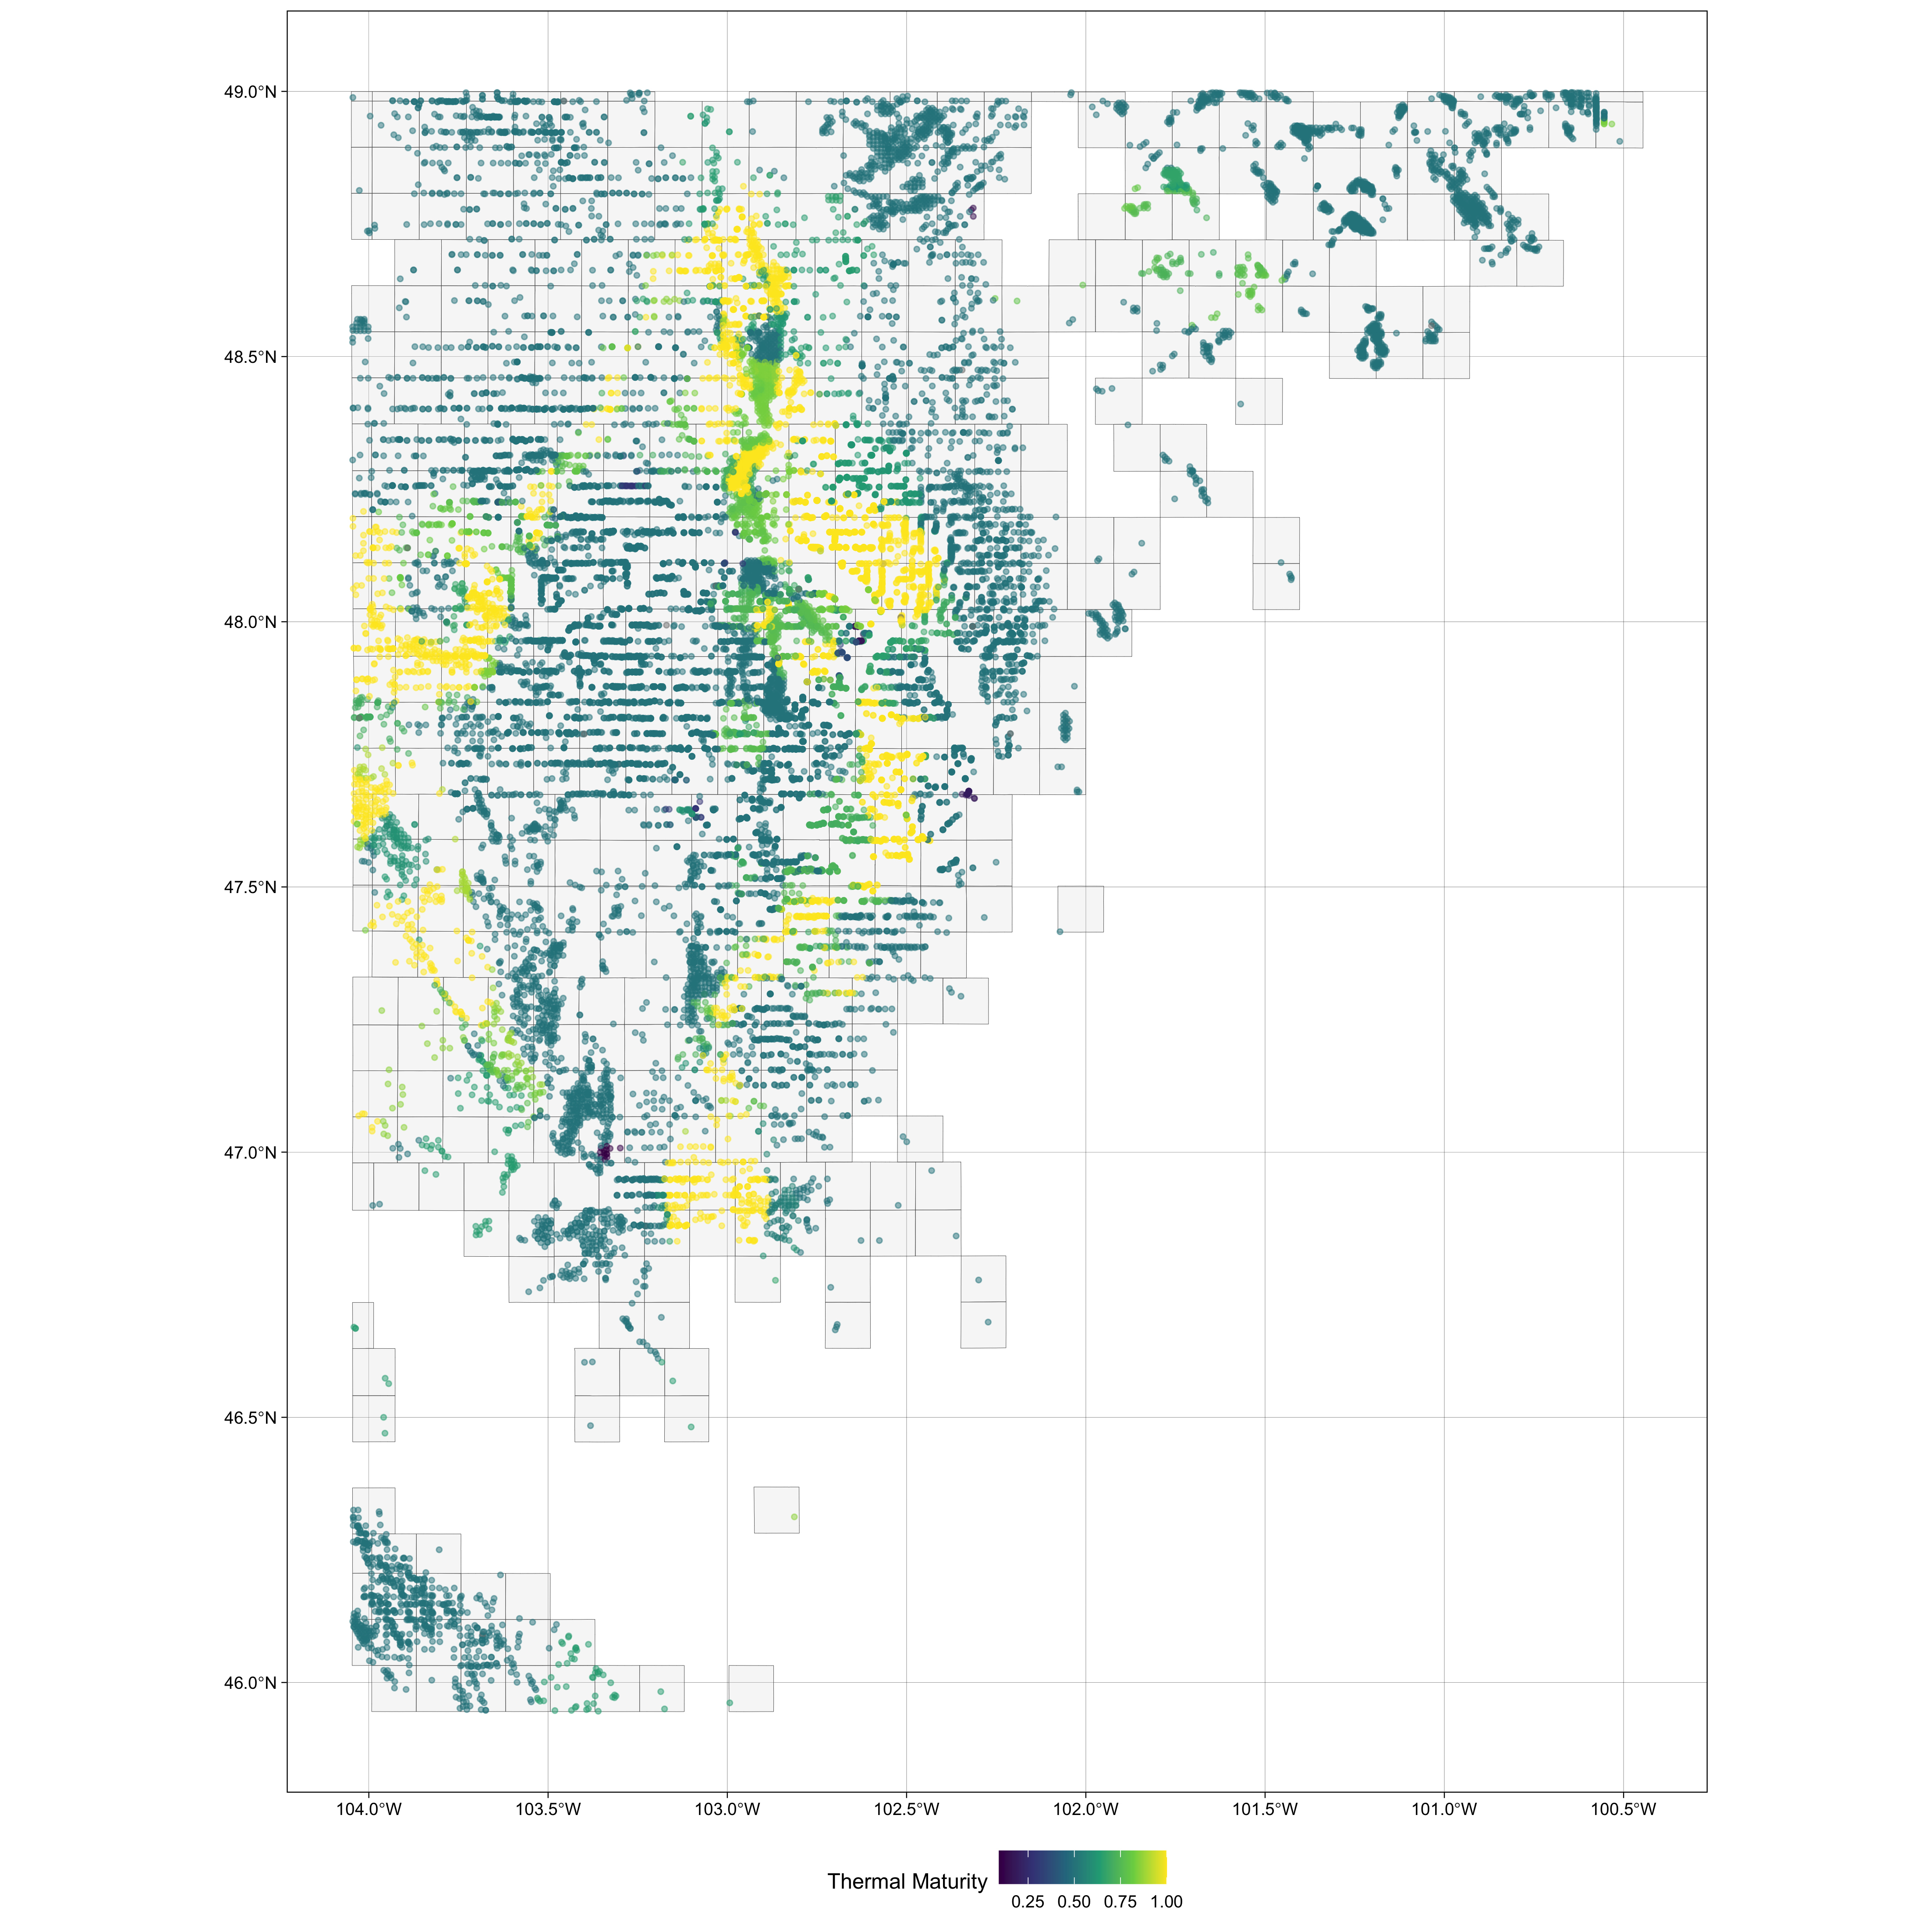
\includegraphics[scale = 0.095]{04_Chapter-3/00A_Figures/Spatial-Distribution_Geological-Characteristics_Thermal-Maturity.png}
        \caption{Spatial Distributions of Geological Characteristics}
        \subcaption*{
            \textit{Note}: 
            This figure depicts the spatial distributions of three geological features---thickness, thermal maturity, and total organic contents---, which are available from the NDGS' geological survey data. In this figure, each dot indicates an individual well. 
        }
        \label{Figure:Spatial-Distributions-of-Geological-Characteristics}
    \end{figure}
% }
\end{landscape}
% \clearpage

\begin{landscape}
%\afterpage{
    \begin{figure}[t!]
        \centering
        \includegraphics[scale = 0.075]{04_Chapter-3/00A_Figures/Robinson-Estimator_Productivity-across-Locations_Discrete.png}
        \caption{Spatial Distribution of the Estimated Geological Characteristic by Year}
        \subcaption*{
            \textit{Note}: 
            This figure illustrates the estimated geologic feature for each horizontal well by year. It is apparent that the share of drilling of horizontal wells with (relatively) small estimates decreased significantly starting in 2014, corresponding to the beginning of the oil price crash.
        }
        \label{Figure:Spatial-Distribution-of-the-Estimated-Geological-Characteristic-by-Year}
    \end{figure}
%}
\end{landscape}
\clearpage

\afterpage{
    \begin{figure}[t!]
        \centering
        \includegraphics[scale = 0.1]{04_Chapter-3/00A_Figures/Cross-Sectional-Approach_Estimates-from-Robinson-Estimator_Time-Trend_Unobservable-Geology.png}
        \caption{Simultaneous Drilling of Horizontal Wells with Heterogeneous Geological Quality}
        \subcaption*{
            \textit{Note}: 
            This figure indicates the estimated geological feature for each horizontal well, depicted as a dot. Those dots definitely suggest the simultaneous drilling of horizontal wells with heterogeneous geological quality. In the figure, percentiles of the estimates, with the 95\% confidence interval of each, are also presented. The dot-dashed line is the time series of the monthly per-barrel spot prices for West Texas Intermediate at Cushing, Oklahoma. Oil prices plunged significantly between 2014 and 2015 and rose gradually. The percentile lines skewed upward, especially lower ones, as of the second half of 2014. 
        }
        \label{Figure:Simultaneous-Drilling-of-Horizontal-Wells-with-Heterogeneous-Geological-Quality}
    \end{figure}
}
\clearpage

\afterpage{
    \begin{figure}[t!]
        \centering
        \includegraphics[scale = 0.095]{04_Chapter-3/00A_Figures/Estimates-from-Robinson-Estimator_By-Firm.png}
        \caption{High Sensitivity of Firm-Level Low-Quality Well Drilling to the Negative Price Shocks in 2014-15}
        \subcaption*{
            \textit{Note}: 
            This figure shows how each of the four firms' drilling activity changed over time. Each dot in the figure indicates an individual well's estimated geological feature. The red line, with the 95\% confidence interval, in each panel demonstrates the average quality of horizontal wells drilled in a month. As illustrated, the firms significantly reduced drilling low-quality well locations since mid-2014, corresponding to the beginning of the oil price plunge.
        }
        \label{Figure:High-Sensitivity-of-Firm-Level-Low-Quality-Well-Drilling}
    \end{figure}
}
\clearpage

\afterpage{
    \begin{figure}[t!]
        \centering
        \includegraphics[scale = 0.11]{04_Chapter-3/00A_Figures/Drilling-over-Time_By-Well-Quality-and-Whether-First-Drilled.png}
        \caption{Held-by-Production vs. Non-Held-by-Production Horizontal Well Drilling}
        \subcaption*{
            \textit{Note}: 
            This figure depicts the drilling of horizontal wells classified into three quality levels. Drilling described in the upper panel is the first in each section, regarded as held-by-production drilling. There was only a limited number of held-by-production drilling between 2015 and 2019. The lower panel indicates all subsequent drilling in sections. The collapse in oil prices between mid-2014 and 2015 made post-held-by-production drilling decrease. Drilling of high-quality well sites was more responsive to the recovery of oil prices from 2016 to 2019. In each panel, the dot-dashed line is the time series of the monthly per-barrel spot prices for West Texas Intermediate at Cushing, Oklahoma.
        }
        \label{Figure:Held-by-Production-vs-Non-Held-by-Production-Horizontal-Well-Drilling}
    \end{figure}
}
\clearpage

\afterpage{
    \begin{figure}[t!]
        \centering
        \includegraphics[scale = 0.20]{04_Chapter-3/00A_Figures/Figure_Equilibrium-Path_Exogenous-Price_Phase-Diagram_pi-by-R.png}
        \includegraphics[scale = 0.20]{04_Chapter-3/00A_Figures/Figure_Equilibrium-Path_Exogenous-Price_Phase-Diagram_Pr-by-R.png}
        \caption{Phase Diagrams for the Social Planner's Problem}
        \subcaption*{
            \textit{Note}: 
            This figure shows two phase diagrams for the social planner's problem. The upper diagram illustrates that the steady state is exactly a saddle point. This figure assumes that a dispersion parameter of $\sigma = 1$, an interest rate of $r = 0.15$, initial reserves of $R_{0} = 1$, additional reserves of $E = 0.05$, and exogenously given constant oil prices of $\bar{p} = 50$. Also, a linear marginal cost function of $c'(D_{t}) = 1 + 5D_{t}$ is assumed.  
        }
        \label{Figure:Phase-Diagram_Saddle-Point}
    \end{figure}
}
\clearpage

\afterpage{
    \begin{figure}[t!]
        \centering
        \includegraphics[scale = 0.15]{04_Chapter-3/00A_Figures/Figure_Equlibrium-Paths_Exogenous-Price.png}
        \caption{Equilibrium Paths under Unexpected Price Shocks}
        \subcaption*{
            \textit{Note}: 
            This figure shows the equilibrium paths for drilling probability, drilling, and undrilled reserves for exogenously given oil prices, including two unanticipated price shocks. This figure assumes the identical parameter values and the marginal cost function utilized to draw the phase diagrams in Figure \ref{Figure:Phase-Diagram_Saddle-Point}.
        }
        \label{Figure:Equilibrium-Paths-under-Unexpected-Price-Shocks}
    \end{figure}
}
\clearpage

\afterpage{
    \begin{figure}[t!]
        \centering
%        \includegraphics[scale = 0.1]{}
        \caption{Heterogeneous Impacts of Unexpected Price Shocks on Equilibrium Paths}
        \subcaption*{
            \textit{Note}: 
            (...)
        }
        \label{Figure:Heterogeneous-Impacts-of-Unexpected-Price-Shocks-on-Equilibrium-Paths}
    \end{figure}
}
\clearpage

\afterpage{
    \begin{figure}[t!]
        \centering
        \includegraphics[scale = 0.14]{04_Chapter-3/00A_Figures/Figure_Reserves-and-Drilling-Paths_Endogenous-and-Exogenous-Prices.png}
        \caption{Time Paths for Drilling and Reserves under Endogenous and Exogenous Oil Prices}
        \subcaption*{
            \textit{Note}: 
            This figure depicts differences in the time paths for drilling and reserves under endogenous and exogenous oil prices. This figure takes the assumptions exploited in Figure \ref{Figure:Phase-Diagram_Saddle-Point}, except the initial stock of $R_{0} = 10$ to magnify the differences. See the text for details.
        }
        \label{Figure:Time-Paths-for-Drilling-and-Reserves-under-Endogenous-and-Exogenous-Oil-Prices}
    \end{figure}
}
\clearpage



% Tables
\setcounter{table}{1}
\afterpage{
    \begin{table}
        \centering
        \caption{Summary Statistics for Wells}
        \label{Table:Summary-Statistics-for-Wells}
        \vspace{0.2cm}
        \begin{adjustbox}{scale = 0.85}
            \begin{tabular}{
                >{\raggedright}m{6.0cm}
                >{\raggedleft}m{2.2cm}
                >{\raggedleft}m{2.2cm}
                >{\raggedleft}m{2.2cm}
                >{\raggedleft}m{2.2cm}
                >{\raggedleft\arraybackslash}m{2.2cm}
            }
                \hline \hline
                \multicolumn{1}{c}{} & \multicolumn{1}{c}{Mean} & \multicolumn{1}{c}{(S.D.)} & \multicolumn{1}{c}{P25} & \multicolumn{1}{c}{P50} & \multicolumn{1}{c}{P75} \\
                \hline
                \underline{Production} &  &  &  &  &  \\
                \hspace{0.2cm} Cumulative Oil Production \ (Bbls) & 211,491.30 & (108,012.00) & 136,811.50 & 193,354.00 & 267,052.20 \\
                \hspace{0.2cm} Cumulative Producing Days \ (Days) & 1,451.37 & (356.58) & 1,343.75 & 1,601.00 & 1,697.00 \\
                \underline{Drilling} &  &  &  &  &  \\
                \hspace{0.2cm} Water \ (Bbls) & 101,716.50 & (249,157.50) & 42,032.75 & 65,856 & 130,219.20 \\
                \hspace{0.2cm} Sand/Proppants \ (Lbs) & 4,553,380.00 & (4,560,985.00) & 2,312,951 & 3,441,914 & 5,543,660.00 \\
                \hspace{0.2cm} Horizontal Drilling \ (Feet) & 23,866.77 & (15,134.08) & 19,276.23 & 20,025.88 & 21,227.25 \\
                \underline{Geological Characteristics} &  &  &  &  &  \\
                \hspace{0.2cm} Thickness \ (Feet) & 44.79 & (13.48) & 37.50 & 44.50 & 44.50 \\
                \hspace{0.2cm} Thermal Maturity & 0.64 & (0.20) & 0.50 & 0.50 & 0.75 \\
                \hspace{0.2cm} Total Organic Content & 13.62 & (1.98) & 12.24 & 13.34 & 15.13 \\
                \hline \hline
            \end{tabular}
        \end{adjustbox}
        \begin{minipage}{15.5cm}
            \small \singlespacing
            \textit{Note}: This table presents summary statistics for horizontal wells in our sample.
        \end{minipage}
    \end{table}
}

\clearpage

